\documentclass[10pt,aspectratio=169]{beamer}

\usetheme{metropolis}
\metroset{sectionpage=none}

\usepackage{amsmath,amssymb,amsfonts}
\usepackage{bm}
\usepackage{booktabs}
\usepackage{tikz}
\usepackage{xcolor}
\usepackage{pgfplots}
\pgfplotsset{compat=1.18}
\usetikzlibrary{arrows.meta, positioning, shapes.geometric, fit, backgrounds,
                decorations.pathreplacing, decorations.markings, calc}

% Useful macros
\newcommand{\T}{\mathcal{T}}
\newcommand{\Hh}{\mathcal{H}}
\newcommand{\E}{\mathbb{E}}
\newcommand{\R}{\mathbb{R}}
\newcommand{\N}{\mathcal{N}}
\newcommand{\indep}{\perp\!\!\!\perp}

\title{Horseshoe Forests for High-Dimensional\\ Causal Survival Analysis}
\subtitle{}
\date{}
\author{Tijn Jacobs \\
\small joint work with Wessel N.\ van Wieringen and St\'ephanie L.\ van der Pas}
\institute{Vrije Universiteit Amsterdam}

\definecolor{myaccent}{HTML}{0077B3}
\setbeamercolor{alerted text}{fg=myaccent}
\setbeamercolor{progress bar}{fg=myaccent}
\setbeamercolor{frametitle}{bg=myaccent, fg=white}
\setbeamercolor{normal text}{fg=black!90, bg=white}

\usepackage{graphicx}
\usepackage{qrcode}
\titlegraphic{%
  \vspace{6.5cm}%
  \hfill
\includegraphics[height=1cm]{VU-logo-CMYK.pdf}%
}

\begin{document}

\maketitle

%=========================================================
% PART 0  -  Opener
%=========================================================

%---------------------------------------------------------
\begin{frame}{Motivating question: pancreatic cancer}
\begin{columns}[T,onlytextwidth]
\begin{column}{0.42\textwidth}
\textbf{Pancreatic ductal adenocarcinoma (PDAC).}
\begin{itemize}
  \item One of the deadliest cancers; median survival $<\,$6 months.
  \item Surgical resection $+$ adjuvant radiotherapy is often the only curative option.
\end{itemize}

\bigskip

\textbf{TCGA-PAAD cohort.}
\begin{itemize}
  \item $n = 130$ resected patients.
  \item 11 clinical covariates $+$ $\sim$3{,}000 gene expressions.
  \item Censoring $\approx 47\%$.
\end{itemize}

\bigskip

\alert{Does adjuvant radiotherapy improve survival, and for whom?}
\end{column}
\begin{column}{0.58\textwidth}
\centering
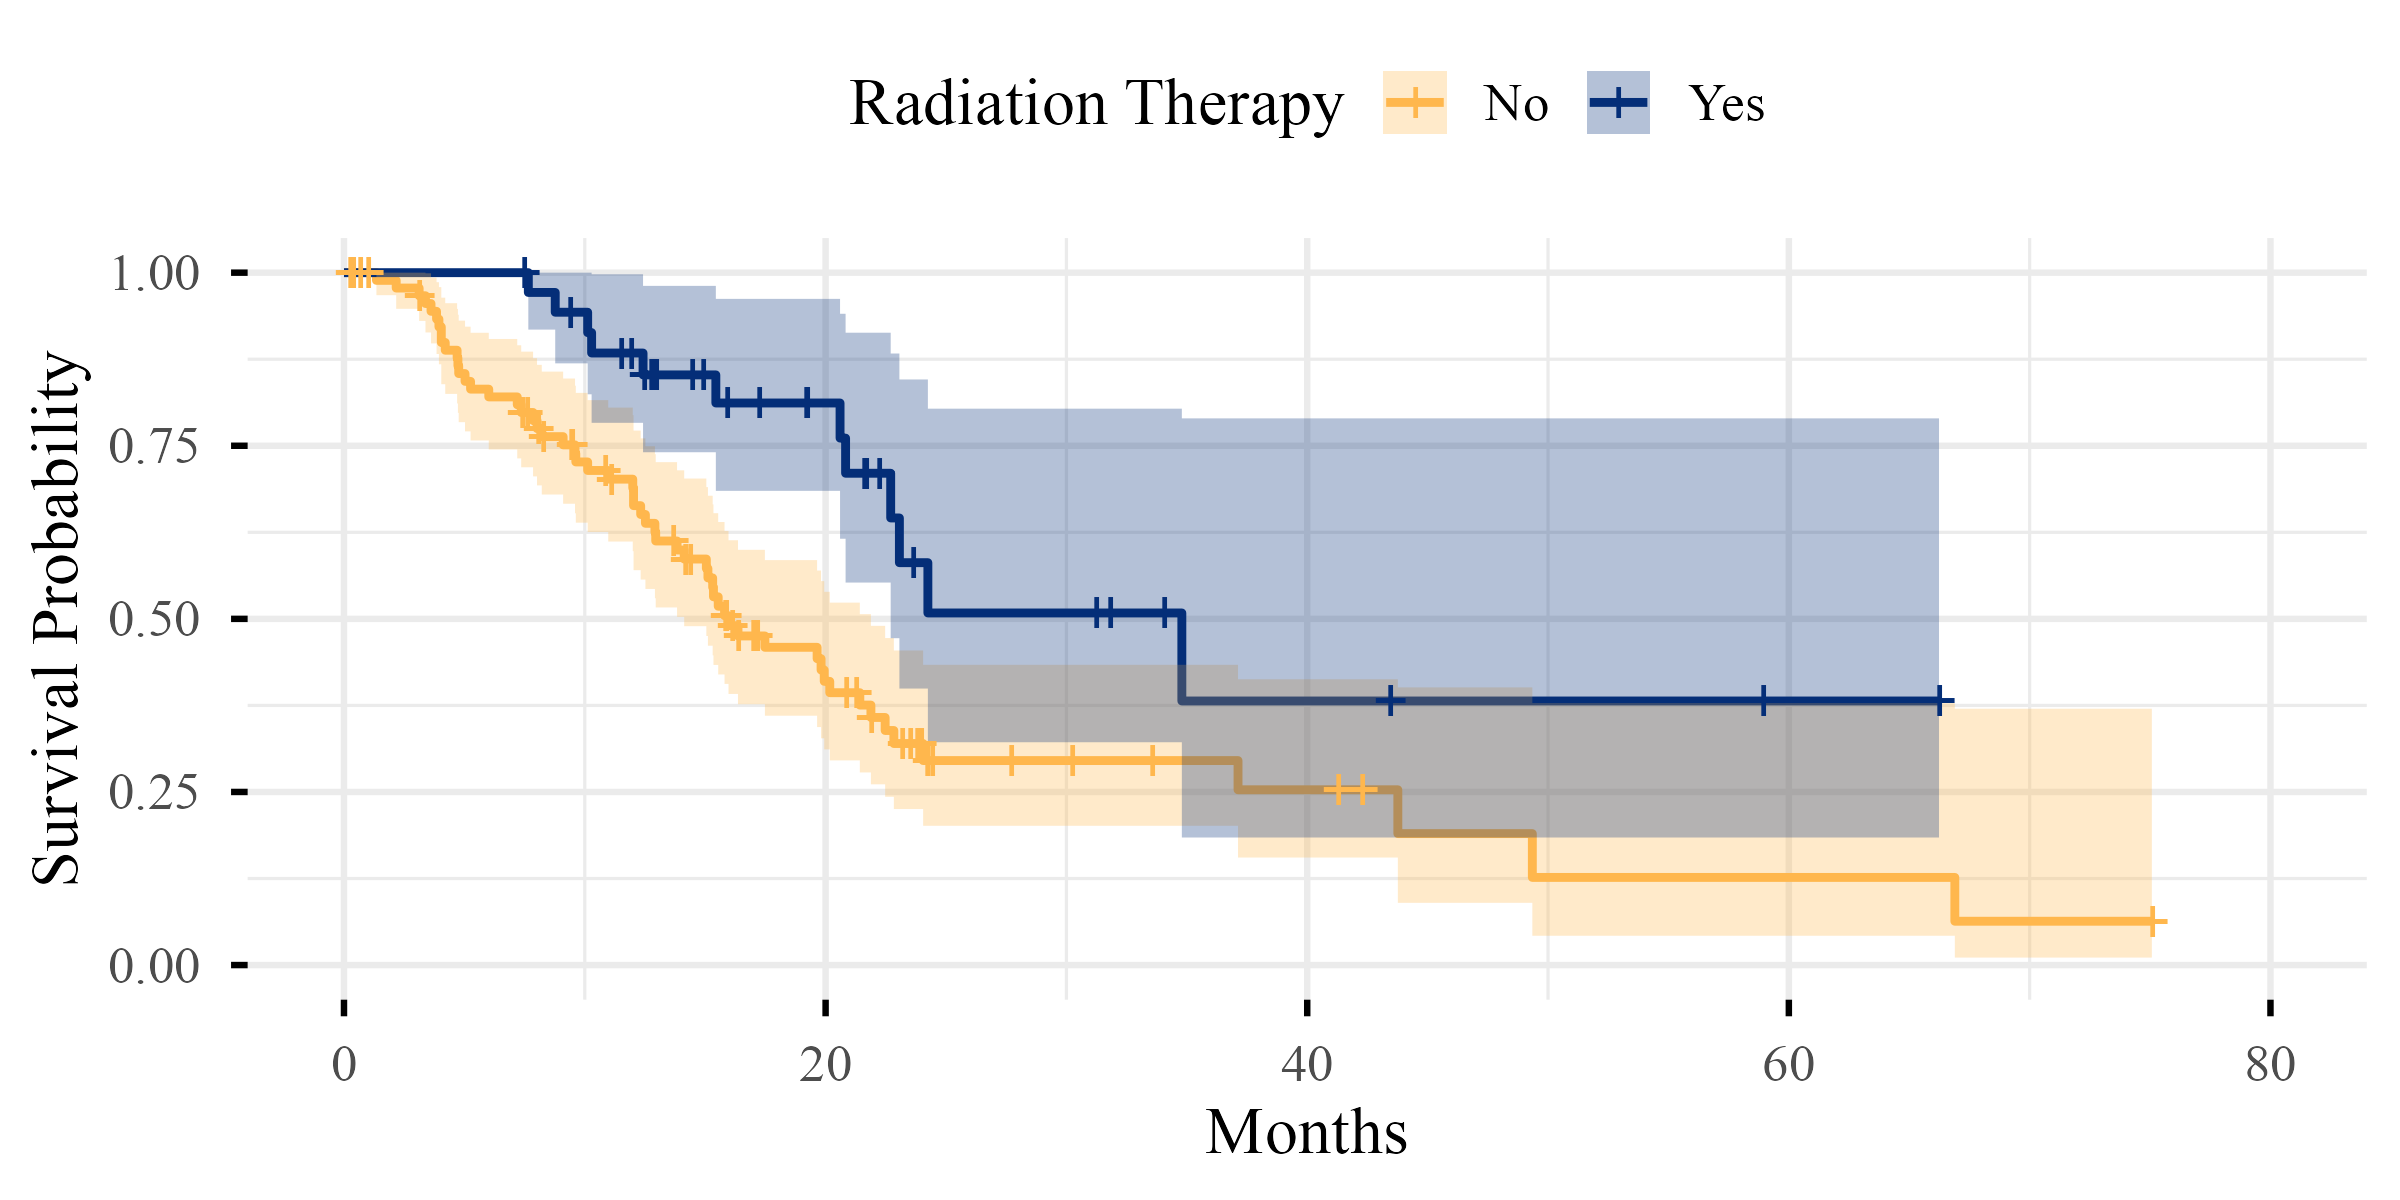
\includegraphics[width=\linewidth]{PDAC_KaplanMeier.png}
\end{column}
\end{columns}
\end{frame}

%=========================================================
\section{Setup}
%=========================================================

%---------------------------------------------------------
\begin{frame}{The setting}
\begin{columns}[T,onlytextwidth]
\begin{column}{0.68\textwidth}
\textbf{Observational survival data} $(Y_i, \delta_i, A_i, X_i)$, $i=1,\ldots,n$:
\begin{itemize}
  \item $Y_i = \min(T_i, C_i)$, $\delta_i = \mathbf{1}\{T_i \le C_i\}$ \quad (right-censored).
  \item $A_i \in \{0,1\}$ \quad (binary, non-randomised).
  \item $X_i \in \R^p$ \quad with $p \gg n$.
\end{itemize}

\bigskip

\textbf{Three sources of difficulty.}
\begin{itemize}
  \item \emph{Observational}: treatment and outcome share causes.
  \item \emph{Censored}: only partial information about $T$.
  \item \emph{High-dimensional}: classical non-parametric tools break down.
\end{itemize}
\end{column}
\begin{column}{0.30\textwidth}
\centering
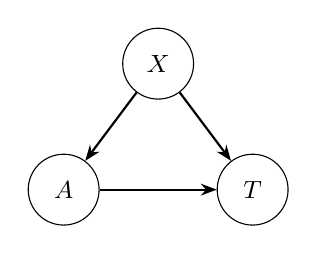
\begin{tikzpicture}[
  every node/.style={circle, draw, minimum size=0.9cm, font=\small},
  arr/.style={-{Stealth[length=2mm]}, thick}
]
\node (X) at (0,1.2)    {$X$};
\node (A) at (-1.2,-0.4) {$A$};
\node (T) at (1.2,-0.4)  {$T$};
\draw[arr] (X) -- (A);
\draw[arr] (X) -- (T);
\draw[arr] (A) -- (T);
\end{tikzpicture}
\end{column}
\end{columns}
\end{frame}

%---------------------------------------------------------
\begin{frame}{Estimands: potential outcomes}
For each individual, imagine \emph{both} treatment counterfactuals:
\[
T(1):\text{ survival under treatment.}\qquad
T(0):\text{ survival under control.}
\]

\textbf{Fundamental problem of causal inference.} Only one is ever observed:
\[
T \;=\; A\, T(1) \;+\; (1 - A)\, T(0).
\]

\bigskip

\textbf{Estimands on the log scale.}
\begin{itemize}
  \item \emph{Average treatment effect:} $\tau \;:=\; \E\!\left[\log T(1) - \log T(0)\right]$.
  \item \emph{Conditional average treatment effect:}
  $\;\tau(x) \;:=\; \E\!\left[\log T(1) - \log T(0)\,\big|\, X = x\right]$.
\end{itemize}

\medskip

\textbf{Goal.} Estimate $\tau(x)$ — how the treatment effect varies across patients.
\end{frame}

%---------------------------------------------------------
\begin{frame}{Intuition: the acceleration factor}
On the log scale, $\tau(x)$ is a difference. Exponentiated, it is a \emph{multiplier on survival time}:
\[
T(1)\,\big|\,X=x \;\;\overset{d}{=}\;\; e^{\tau(x)} \cdot T(0)\,\big|\,X=x.
\]

\begin{columns}[T,onlytextwidth]
\begin{column}{0.5\textwidth}
\medskip
\textbf{Reading the picture.}
\begin{itemize}
  \item Treatment \emph{stretches the patient's clock} by a factor $e^{\tau(x)}$.
  \item $e^{\tau(x)} = 2 \;\Rightarrow\;$ median survival doubles.
  \item Same shape, different time scale.
\end{itemize}

\bigskip

\textbf{Contrast with the hazard ratio.}
\begin{itemize}
  \item HR multiplies \emph{hazards}.
  \item Acceleration factor multiplies \emph{time itself}.
\end{itemize}
\end{column}
\begin{column}{0.5\textwidth}
\centering
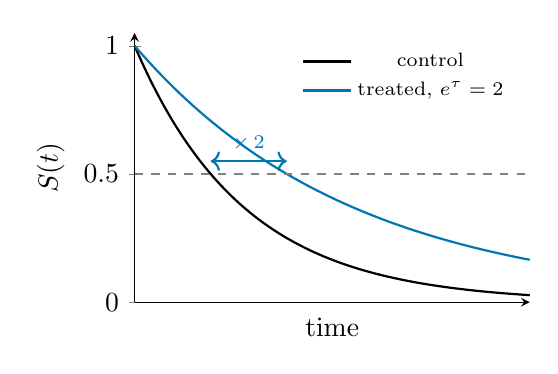
\begin{tikzpicture}
\begin{axis}[
  width=6.6cm, height=5cm,
  xlabel={time}, ylabel={$S(t)$},
  xmin=0, xmax=12, ymin=0, ymax=1.05,
  xtick=\empty, ytick={0,0.5,1},
  legend pos=north east,
  legend style={font=\scriptsize, draw=none},
  axis lines=left,
]
\addplot[domain=0:12, samples=200, thick, black]    {exp(-0.30*x)};
\addlegendentry{control}
\addplot[domain=0:12, samples=200, thick, myaccent] {exp(-0.15*x)};
\addlegendentry{treated, $e^{\tau}=2$}
\draw[dashed, gray] (axis cs:0,0.5) -- (axis cs:12,0.5);
\draw[<->, thick, myaccent]
  (axis cs:2.31,0.55) -- (axis cs:4.62,0.55)
  node[midway,above,font=\scriptsize,text=myaccent]{$\times\,2$};
\end{axis}
\end{tikzpicture}
\end{column}
\end{columns}
\end{frame}

%---------------------------------------------------------
\begin{frame}{Why AFT, and not Cox?}
The default for survival is Cox. Three reasons to switch here:

\medskip

\textbf{1.~Interpretability.} The acceleration factor $e^{\tau(x)}$ acts on the \emph{time scale}, not on hazards. A doubling of expected survival is a directly clinically meaningful statement.

\medskip

\textbf{2.~Collapsibility.}
\[
\E_X\!\bigl[e^{\tau(X)}\bigr] \;=\; \text{marginal acceleration factor.}
\]
We can meaningfully \emph{average} CATEs to get the ATE. The hazard ratio is \emph{non-collapsible} — marginal HR $\neq$ average of conditional HRs.

\medskip

\textbf{3.~Robustness.} Hougaard~(1999): the AFT model is robust to omitted independent covariates; partial-hazard models are not.

\medskip

\alert{Throughout, we model $\log T$.}
\end{frame}

%=========================================================
\section{Identification}
%=========================================================

%---------------------------------------------------------
\begin{frame}{Unconfoundedness, intuitively}
\begin{columns}[T,onlytextwidth]
\begin{column}{0.55\textwidth}
\textbf{The worry.} Sicker patients may be more likely (or less likely) to be treated. A naive treated-versus-untreated comparison conflates the \emph{treatment effect} with \emph{baseline differences}.

\bigskip

\textbf{Unconfoundedness.}
\[
T(a) \;\indep\; A \;\Big|\; X, \qquad a \in \{0,1\}.
\]
\emph{``Within each value of $X$, treatment looks as if randomised.''}

\bigskip

\textbf{Operationally.} Imagine \alert{matching like-for-like}: for any pair of patients with $X_i = X_j$, the only systematic difference between them is the treatment they received.
\end{column}
\begin{column}{0.40\textwidth}
\centering
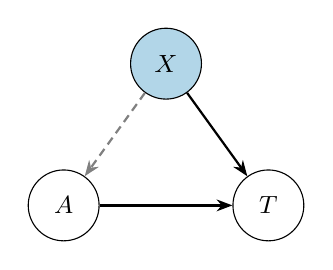
\begin{tikzpicture}[
  every node/.style={circle, draw, minimum size=0.9cm, font=\small},
  arr/.style={-{Stealth[length=2mm]}, thick}
]
\node[fill=myaccent!30] (X) at (0,1.4)    {$X$};
\node (A) at (-1.3,-0.4) {$A$};
\node (T) at (1.3,-0.4)  {$T$};
\draw[arr, gray, densely dashed] (X) -- (A);
\draw[arr] (X) -- (T);
\draw[arr] (A) -- (T);
\end{tikzpicture}

\vspace{0.4cm}
{\footnotesize Conditioning on $X$ (filled node) ``cuts'' the dashed back-door arrow. Within each $X$-stratum, the $A$--$T$ contrast is causal.}
\end{column}
\end{columns}
\end{frame}

%---------------------------------------------------------
\begin{frame}{What goes wrong if a confounder is missed?}
\begin{columns}[T,onlytextwidth]
\begin{column}{0.55\textwidth}
Now suppose we adjust for $X$ but \emph{miss} an unmeasured confounder $U$:

\bigskip

\begin{itemize}
  \item The back-door path $A \leftarrow U \rightarrow T$ remains open.
  \item Naive comparison still picks up the $U$ effect.
  \item \alert{Estimate is biased — even with infinite data.}
\end{itemize}

\bigskip

\textbf{Practical consequence in high dimensions.}\\
We dare not drop covariates aggressively: a dropped variable may be a confounder.

\bigskip

This motivates a regularisation strategy that \alert{keeps every covariate in the model}.
\end{column}
\begin{column}{0.40\textwidth}
\centering
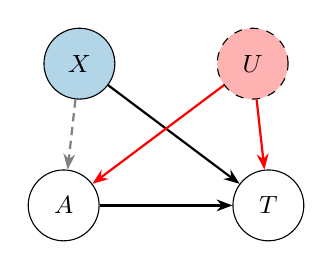
\begin{tikzpicture}[
  every node/.style={circle, draw, minimum size=0.9cm, font=\small},
  arr/.style={-{Stealth[length=2mm]}, thick}
]
\node[fill=myaccent!30] (X) at (-1.1,1.4)  {$X$};
\node[fill=red!30,      dashed] (U) at (1.1,1.4)   {$U$};
\node (A) at (-1.3,-0.4) {$A$};
\node (T) at (1.3,-0.4)  {$T$};
\draw[arr, gray, densely dashed] (X) -- (A);
\draw[arr] (X) -- (T);
\draw[arr, red] (U) -- (A);
\draw[arr, red] (U) -- (T);
\draw[arr] (A) -- (T);
\end{tikzpicture}

\vspace{0.4cm}
{\footnotesize The unmeasured $U$ leaves an open back-door path $A \leftarrow U \rightarrow T$.}
\end{column}
\end{columns}
\end{frame}

%---------------------------------------------------------
\begin{frame}{The remaining identification assumptions}
\textbf{SUTVA.} No interference between units; well-defined potential outcomes. Implies $T = A\,T(1) + (1-A)\,T(0)$.

\bigskip

\textbf{Positivity.} For every $x$, both treatment arms have positive probability:
\[
0 \;<\; e(x) \;:=\; P(A=1 \mid X = x) \;<\; 1.
\]
In $p \gg n$ regimes, this can only hold in a lower-dimensional confounding subspace — a working assumption we cannot verify directly.

\bigskip

\textbf{Independent censoring} (familiar):
\[
C(a) \;\indep\; T(a) \;\Big|\; X, A.
\]
This makes the distribution of $T \mid X, A$ identifiable from $(Y, \delta)$.

\bigskip

Under SUTVA $+$ unconfoundedness $+$ positivity $+$ independent censoring, $\tau(x)$ is identified from the observed data.
\end{frame}

%=========================================================
\section{A quick Bayesian refresher}
%=========================================================

%---------------------------------------------------------
\begin{frame}{Bayes in one slide: priors regularise}
For a single observation $y \sim \N(\mu, \sigma^2)$ with prior $\mu \sim \N(0, \kappa^2)$:
\[
\mu \mid y \;\sim\; \N\!\left(\underbrace{\tfrac{\kappa^2}{\kappa^2+\sigma^2}}_{\text{shrinkage weight}}\!\cdot y,\;\;\tfrac{\kappa^2\sigma^2}{\kappa^2+\sigma^2}\right).
\]

\begin{columns}[T,onlytextwidth]
\begin{column}{0.50\textwidth}
\medskip
\textbf{Three things to take away.}
\begin{itemize}
  \item The posterior is a \emph{distribution}, not a point estimate.
  \item The posterior mean is the MLE \emph{pulled toward the prior mean} — the prior \alert{regularises}.
  \item A tight prior shrinks more; a vague prior shrinks less.
\end{itemize}

\bigskip

\textbf{Slogan.} A Bayesian model regularises for free, and the posterior carries its own uncertainty.
\end{column}
\begin{column}{0.50\textwidth}
\centering
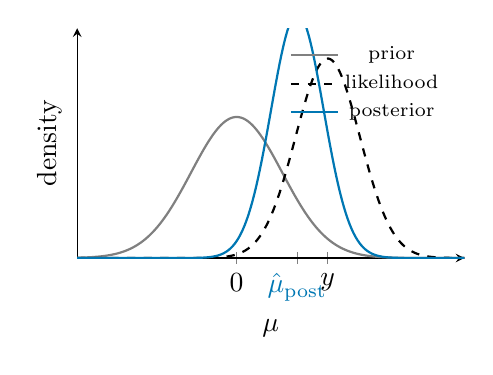
\begin{tikzpicture}
\begin{axis}[
  width=6.5cm, height=4.5cm,
  xlabel={$\mu$}, ylabel={density},
  xmin=-3.5, xmax=5, ymin=0, ymax=0.65,
  xtick={0,1.33,2}, xticklabels={$0$,\textcolor{myaccent}{$\hat\mu_{\text{post}}$},$y$},
  ytick=\empty,
  legend pos=north east,
  legend style={font=\scriptsize, draw=none, fill=none},
  axis lines=left,
]
% prior:  N(0,1)
\addplot[domain=-3.5:5, samples=200, thick, gray] {0.3989*exp(-x*x/2)};
\addlegendentry{prior}
% likelihood (treated as N(y, 0.5))
\addplot[domain=-3.5:5, samples=200, thick, dashed, black] {0.5642*exp(-(x-2)^2/(2*0.5))};
\addlegendentry{likelihood}
% posterior:  N(2/1.5, 1/3)
\addplot[domain=-3.5:5, samples=200, thick, myaccent] {0.6909*exp(-(x-1.333)^2/(2*0.333))};
\addlegendentry{posterior}
\end{axis}
\end{tikzpicture}
\end{column}
\end{columns}
\end{frame}

%---------------------------------------------------------
\begin{frame}{Posterior inference via MCMC}
For models we cannot integrate by hand, we \emph{sample} from the posterior.

\bigskip

\begin{columns}[T,onlytextwidth]
\begin{column}{0.55\textwidth}
\textbf{Markov chain Monte Carlo (MCMC).}
\begin{itemize}
  \item Build a Markov chain whose stationary distribution is the posterior.
  \item Run the chain. Discard burn-in.
  \item Remaining draws are (correlated) samples from the posterior.
\end{itemize}

\bigskip

\textbf{Summarising the posterior.}
\begin{itemize}
  \item Posterior mean $\approx$ average of draws.
  \item \alert{95\% credible interval} $\approx$ 2.5\%--97.5\% sample quantiles.
\end{itemize}

\smallskip
``With 95\% posterior probability, $\tau$ lies in this interval.''
\end{column}
\begin{column}{0.45\textwidth}
\centering
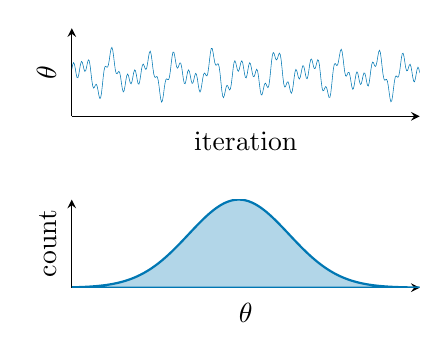
\begin{tikzpicture}
\begin{axis}[
  name=trace,
  width=6cm, height=2.7cm,
  xlabel={iteration}, ylabel={$\theta$},
  xmin=0, xmax=2000, ymin=0.0, ymax=2.5,
  ytick=\empty, xtick=\empty,
  axis lines=left,
]
\addplot[myaccent, very thin, samples=400, domain=0:2000]
  {1.2 + 0.35*sin(deg(x/30)) + 0.25*cos(deg(x/19+1))
        + 0.20*sin(deg(x/7))};
\end{axis}
\begin{axis}[
  width=6cm, height=2.7cm,
  at={(trace.below south west)}, anchor=above north west,
  yshift=-0.5cm,
  xlabel={$\theta$}, ylabel={count},
  xmin=0.0, xmax=2.5, ymin=0,
  ytick=\empty, xtick=\empty,
  axis lines=left,
]
\addplot[domain=0:2.5, samples=200, fill=myaccent!30, draw=myaccent, thick]
  {2.6*exp(-(x-1.2)^2/(2*0.13))} \closedcycle;
\end{axis}
\end{tikzpicture}
\end{column}
\end{columns}
\end{frame}

%=========================================================
\section{A causal AFT model}
%=========================================================

%---------------------------------------------------------
\begin{frame}{The AFT decomposition}
We split log event times into a prognostic and a treatment-effect component:
\[
\log T(a)
\;=\;
\underbrace{f\bigl(x, \hat e(x)\bigr)}_{\text{prognostic}}
\;+\;
\underbrace{a \cdot \tau(x)}_{\text{treatment effect}}
\;+\;
\varepsilon,
\qquad \varepsilon \sim \N(0, \sigma^2).
\]

\bigskip

\textbf{Two regression functions to learn.}
\begin{itemize}
  \item $f(x, \hat e(x))$: prognostic baseline; includes the \emph{estimated} propensity score $\hat e(x)$ as a balancing covariate (Hahn et al., 2020). Plugging $\hat e$ in avoids feedback between the propensity and the outcome models.
  \item $\tau(x)$: heterogeneous treatment effect — our object of interest.
\end{itemize}

\bigskip

\textbf{Plan.} Place a flexible Bayesian tree-ensemble prior on each of $f$ and $\tau$, \emph{separately}.
\end{frame}

%=========================================================
\section{Trees and BART}
%=========================================================

%---------------------------------------------------------
\begin{frame}{One tree is just a partition}
\begin{center}
\begin{minipage}[c]{0.40\linewidth}
  \centering
  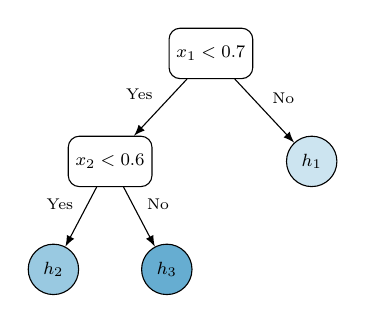
\begin{tikzpicture}[
        scale=0.8, transform shape,
        box/.style={rectangle, draw, rounded corners, align=center,
                    minimum height=8mm, minimum width=13mm, font=\footnotesize},
        leaf/.style={circle, draw, align=center, minimum size=8mm, font=\footnotesize},
        line/.style={-latex}
    ]
    \node [box] (root) {$x_1 < 0.7$};
    \node [box, below=0.9cm of root, xshift=-1.6cm] (left) {$x_2 < 0.6$};
    \node [leaf, fill=myaccent!20, below=0.9cm of root, xshift=1.6cm] (h1) {$h_1$};
    \node [leaf, fill=myaccent!40, below=0.9cm of left, xshift=-0.9cm] (h2) {$h_2$};
    \node [leaf, fill=myaccent!60, below=0.9cm of left, xshift=0.9cm] (h3) {$h_3$};
    \draw[line] (root) -- (left)  node[midway, above left,  font=\scriptsize] {Yes};
    \draw[line] (root) -- (h1)    node[midway, above right, font=\scriptsize] {No};
    \draw[line] (left) -- (h2)    node[midway, above left,  font=\scriptsize] {Yes};
    \draw[line] (left) -- (h3)    node[midway, above right, font=\scriptsize] {No};
  \end{tikzpicture}
\end{minipage}\hfill
\begin{minipage}[c]{0.08\linewidth}
  \centering
  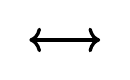
\begin{tikzpicture}\draw[<->, very thick] (0,0) -- (0.9,0);\end{tikzpicture}
\end{minipage}\hfill
\begin{minipage}[c]{0.40\linewidth}
  \centering
  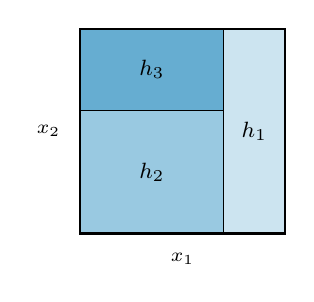
\begin{tikzpicture}[scale=2.6]
    \fill[myaccent!20] (0.7, 0) rectangle (1, 1);
    \fill[myaccent!40] (0, 0)   rectangle (0.7, 0.6);
    \fill[myaccent!60] (0, 0.6) rectangle (0.7, 1);
    \draw[thick] (0, 0) rectangle (1, 1);
    \draw[thin] (0.7, 0) -- (0.7, 1);
    \draw[thin] (0, 0.6) -- (0.7, 0.6);
    \node[below, font=\scriptsize] at (0.5, -0.05) {$x_1$};
    \node[left,  font=\scriptsize] at (-0.05, 0.5) {$x_2$};
    \node[font=\footnotesize] at (0.85, 0.5) {$h_1$};
    \node[font=\footnotesize] at (0.35, 0.3) {$h_2$};
    \node[font=\footnotesize] at (0.35, 0.8) {$h_3$};
  \end{tikzpicture}
\end{minipage}
\end{center}

\bigskip

\textbf{Each tree.} A piecewise-constant function on a partition of $\R^p$. Same idea as CART — and as the trees inside a random forest.
\end{frame}

%---------------------------------------------------------
\begin{frame}{BART: a sum of \emph{weak} learners}
\textbf{Random forest.} A handful of \emph{deep} trees fit greedily, then averaged. Variance reduction through bagging.

\bigskip

\textbf{BART (Bayesian Additive Regression Trees).} A \emph{sum} of $m = 200$ \emph{shallow} trees:
\[
g(x) \;=\; \sum_{j=1}^{m} g(x;\, \T_j, \Hh_j).
\]
\begin{itemize}
  \item Each tree is a \alert{weak learner} — it accounts for only a small piece of the signal.
  \item Trees correct each other's residuals: closer in spirit to boosting than to bagging.
  \item Fit by sampling from a posterior, not by greedy splitting.
\end{itemize}

\bigskip

\textbf{Where does regularisation come from?} The Bayesian prior — explicitly favouring small, shallow trees with small step heights.
\end{frame}

%---------------------------------------------------------
\begin{frame}{The standard BART prior}
For each tree, the prior factorises as
\[
p(\T_j, \Hh_j) \;=\; p_\T(\T_j)\; p_\Hh(\Hh_j \mid \T_j).
\]

\textbf{Structure prior $p_\T$.} A depth-penalised Galton--Watson branching process:
\[
P(\text{node at depth } d \text{ splits}) \;=\; a\,(1 + d)^{-b}.
\]
Discourages deep trees; the splitting variable and split point are chosen uniformly.

\bigskip

\textbf{Step-height prior $p_\Hh$.} Independent Gaussians:
\[
h_{j\ell} \;\sim\; \N\!\bigl(0, 1/(4\sqrt{m})\bigr).
\]
Variance scaled by $1/\sqrt{m}$ so the sum stays in the observed response range.

\bigskip

\alert{All standard-BART regularisation lives in \emph{where the splits go}.}
\end{frame}

%---------------------------------------------------------
\begin{frame}{Where could you regularise a tree ensemble?}
Two natural places:

\bigskip

\begin{enumerate}
  \item \textbf{In the tree structure $\T_j$.}
  \medskip

  Depth penalty, sparse split rules, Dirichlet on splitting variables (DART, Soft-BART, Shrinkage BCF, \ldots).
  \medskip

  \item \textbf{In the step heights $\Hh_j$.}
  \medskip

  Shrink the \emph{magnitudes} of the local effects.
\end{enumerate}

\bigskip

Existing high-dimensional work focuses on (1).
\medskip

\alert{Our proposal: regularise through (2), with a horseshoe prior on step heights.}
\end{frame}

%=========================================================
\section{The horseshoe prior}
%=========================================================

%---------------------------------------------------------
\begin{frame}{Why shrinkage matters in high dimensions}
With $p \gg n$, an unregularised estimator fits noise as eagerly as signal.

\bigskip

\centering
\begin{tikzpicture}[scale=1.0]
% Axis
\draw[thick, ->] (-0.2, 0) -- (11, 0) node[right, font=\scriptsize] {coordinate $j$};
% True coefficients (spike-and-slab pattern)
\foreach \i/\y in {1/0.10, 2/0.05, 3/-0.05, 4/0.00, 5/2.40, 6/-0.10,
                   7/0.05, 8/-1.90, 9/0.00, 10/0.10} {
  \draw[fill=black, draw=none] (\i, 0) rectangle (\i+0.18, \y);
}
\node[font=\scriptsize] at (-0.6, 1.4) {\textbf{truth}};
% Vertical separator
\draw[gray, dashed] (-0.4, -1.5) -- (-0.4, 3.0);
\end{tikzpicture}

\vspace{0.4cm}
\begin{itemize}
  \item \textbf{MLE / no shrinkage:} unbiased but high-variance — noise contaminates every coordinate.
  \item \textbf{Ridge:} stable, but shrinks the large signals \emph{just as much} as the noise.
  \item \textbf{Lasso:} sets small coefficients to exactly zero, but tends to \emph{also} attenuate the large ones.
\end{itemize}

\medskip
\alert{We want a prior that shrinks the noise to zero \emph{and} leaves the signals nearly untouched.}
\end{frame}

%---------------------------------------------------------
\begin{frame}{The horseshoe density}
\begin{columns}[T,onlytextwidth]
\begin{column}{0.45\textwidth}
\vspace{0.3cm}
The horseshoe prior on a coefficient $\theta$:
\[
\theta \mid \lambda, \gamma \;\sim\; \N(0, \lambda^2 \gamma^2),
\]
\[
\lambda, \gamma \;\sim\; \mathcal{C}^+(0,1).
\]

\medskip

\textbf{Two defining features:}
\begin{itemize}
  \item \alert{Pole at zero} — strong shrinkage of noise.
  \item \alert{Heavy tails} — large signals are \emph{not} shrunk.
\end{itemize}

\smallskip

Gaussian has neither; Lasso has the spike but not the tails.
\end{column}
\begin{column}{0.55\textwidth}
\centering
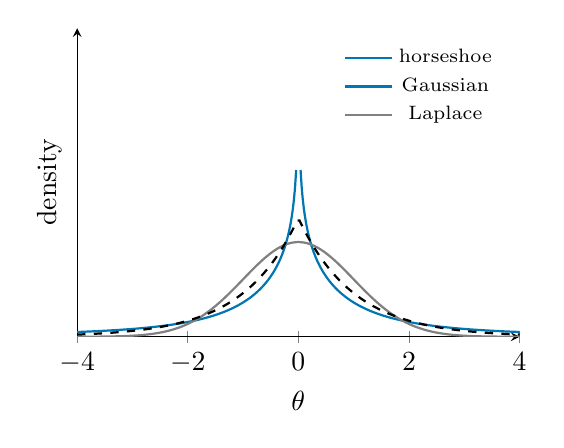
\begin{tikzpicture}
\begin{axis}[
  width=7.2cm, height=5.5cm,
  xlabel={$\theta$}, ylabel={density},
  xmin=-4, xmax=4, ymin=0, ymax=1.3,
  ytick=\empty,
  legend pos=north east,
  legend style={font=\scriptsize, draw=none, fill=none},
  axis lines=left,
]
% horseshoe approximation: 1/(2 pi^(3/2)) * log(1 + 4/x^2)
\addplot[domain=-4:-0.04, samples=200, thick, myaccent]
  {ln(1 + 4/(x*x)) / (2*3.14159^1.5)};
\addplot[domain=0.04:4, samples=200, thick, myaccent]
  {ln(1 + 4/(x*x)) / (2*3.14159^1.5)};
\addlegendentry{horseshoe}
% Gaussian
\addplot[domain=-4:4, samples=200, thick, gray]
  {0.3989*exp(-x*x/2)};
\addlegendentry{Gaussian}
% Laplace (Lasso)
\addplot[domain=-4:4, samples=200, thick, dashed, black]
  {0.5*exp(-abs(x))};
\addlegendentry{Laplace}
\end{axis}
\end{tikzpicture}
\end{column}
\end{columns}
\end{frame}

%---------------------------------------------------------
\begin{frame}{Why ``horseshoe''? The shape of the shrinkage weight}
Reparametrise: define $\kappa = 1 / (1 + \lambda^2 \gamma^2) \in [0,1]$. Then the posterior mean is
\[
\widehat\theta \;=\; (1 - \kappa)\,\bar y.
\]
\[
\kappa = 1 \;\Rightarrow\; \text{full shrinkage to 0}; \qquad
\kappa = 0 \;\Rightarrow\; \text{no shrinkage}.
\]

\begin{columns}[T,onlytextwidth]
\begin{column}{0.55\textwidth}
\vspace{0.4cm}
\textbf{Under the horseshoe prior:}
\[
\kappa \;\sim\; \mathrm{Beta}\!\left(\tfrac{1}{2}, \tfrac{1}{2}\right).
\]

\bigskip

\textbf{This density is U-shaped.} It puts mass at the two extremes:
\begin{itemize}
  \item $\kappa \approx 1$: ``this is noise, kill it.''
  \item $\kappa \approx 0$: ``this is signal, let it through.''
\end{itemize}

\smallskip

\alert{The Bayesian model picks $\kappa$ \emph{per coefficient}, from the data.}
\end{column}
\begin{column}{0.45\textwidth}
\centering
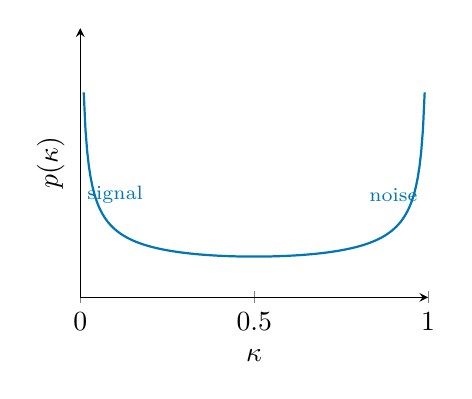
\begin{tikzpicture}
\begin{axis}[
  width=6cm, height=5cm,
  xlabel={$\kappa$}, ylabel={$p(\kappa)$},
  xmin=0, xmax=1, ymin=0, ymax=4.2,
  ytick=\empty,
  xtick={0,0.5,1},
  axis lines=left,
]
\addplot[domain=0.01:0.99, samples=200, thick, myaccent]
  {1 / (3.14159 * sqrt(x*(1-x)))};
\node[font=\scriptsize, text=myaccent] at (axis cs: 0.1, 1.6) {signal};
\node[font=\scriptsize, text=myaccent] at (axis cs: 0.9, 1.6) {noise};
\end{axis}
\end{tikzpicture}

\vspace{-0.2cm}
{\footnotesize That U-shape is the ``horseshoe''.}
\end{column}
\end{columns}
\end{frame}

%---------------------------------------------------------
\begin{frame}{Two regimes, decided coefficient by coefficient}
\begin{columns}[T,onlytextwidth]
\begin{column}{0.50\textwidth}
\centering
\textbf{Signal regime: $\kappa \to 0$}

\bigskip

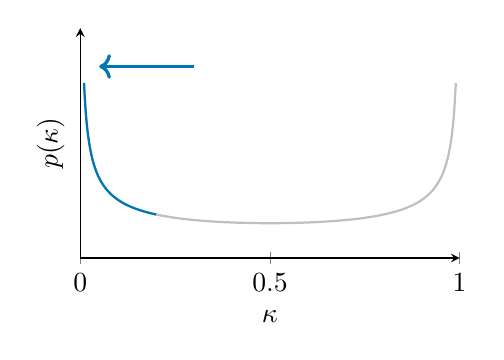
\begin{tikzpicture}
\begin{axis}[
  width=6.4cm, height=4.5cm,
  xlabel={$\kappa$}, ylabel={$p(\kappa)$},
  xmin=0, xmax=1, ymin=0, ymax=4.2,
  ytick=\empty,
  xtick={0,0.5,1},
  axis lines=left,
]
\addplot[domain=0.01:0.99, samples=200, thick, gray!50]
  {1 / (3.14159 * sqrt(x*(1-x)))};
\addplot[domain=0.01:0.20, samples=200, thick, myaccent]
  {1 / (3.14159 * sqrt(x*(1-x)))};
\draw[->, myaccent, very thick]
  (axis cs:0.30,3.5) -- (axis cs:0.05,3.5);
\end{axis}
\end{tikzpicture}

{\footnotesize \(\widehat\theta \approx \bar y\) — no shrinkage.}
\end{column}
\begin{column}{0.50\textwidth}
\centering
\textbf{Noise regime: $\kappa \to 1$}

\bigskip

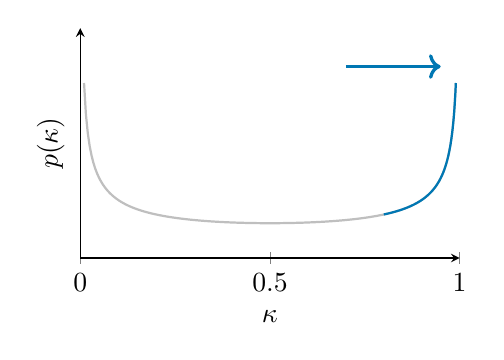
\begin{tikzpicture}
\begin{axis}[
  width=6.4cm, height=4.5cm,
  xlabel={$\kappa$}, ylabel={$p(\kappa)$},
  xmin=0, xmax=1, ymin=0, ymax=4.2,
  ytick=\empty,
  xtick={0,0.5,1},
  axis lines=left,
]
\addplot[domain=0.01:0.99, samples=200, thick, gray!50]
  {1 / (3.14159 * sqrt(x*(1-x)))};
\addplot[domain=0.80:0.99, samples=200, thick, myaccent]
  {1 / (3.14159 * sqrt(x*(1-x)))};
\draw[->, myaccent, very thick]
  (axis cs:0.70,3.5) -- (axis cs:0.95,3.5);
\end{axis}
\end{tikzpicture}

{\footnotesize \(\widehat\theta \approx 0\) — full shrinkage.}
\end{column}
\end{columns}

\bigskip

\alert{The horseshoe is built to live at the two ends of $\kappa$.} It does not compromise like Lasso or ridge.

\smallskip
{\footnotesize (van der Pas et al., 2014, 2017: near-minimax posterior contraction over sparsity classes.)}
\end{frame}

%---------------------------------------------------------
\begin{frame}{Global--local: a global rule with local exceptions}
\[
h_\ell \mid \lambda_\ell^2, \gamma^2 \;\sim\; \N(0, \lambda_\ell^2\, \gamma^2), \qquad
\lambda_\ell \sim \mathcal{C}^+(0,1), \quad \gamma \sim \mathcal{C}^+(0,1).
\]

\bigskip

\begin{columns}[T,onlytextwidth]
\begin{column}{0.55\textwidth}
\textbf{Two layers of shrinkage.}
\begin{itemize}
  \item \textbf{Global $\gamma$.} Pulls \emph{everything} towards zero. Learned: if the world is sparse, $\gamma$ becomes small.
  \item \textbf{Local $\lambda_\ell$.} Lets individual coordinates \emph{escape} the global pull when the data demand it.
\end{itemize}

\bigskip

\emph{``Shrink globally, recover locally.''}

\bigskip

\textbf{Why this beats one-size-fits-all.} A single ridge $\lambda$ can either over-shrink the signals or under-shrink the noise. Horseshoe avoids the trade-off.
\end{column}
\begin{column}{0.45\textwidth}
\centering
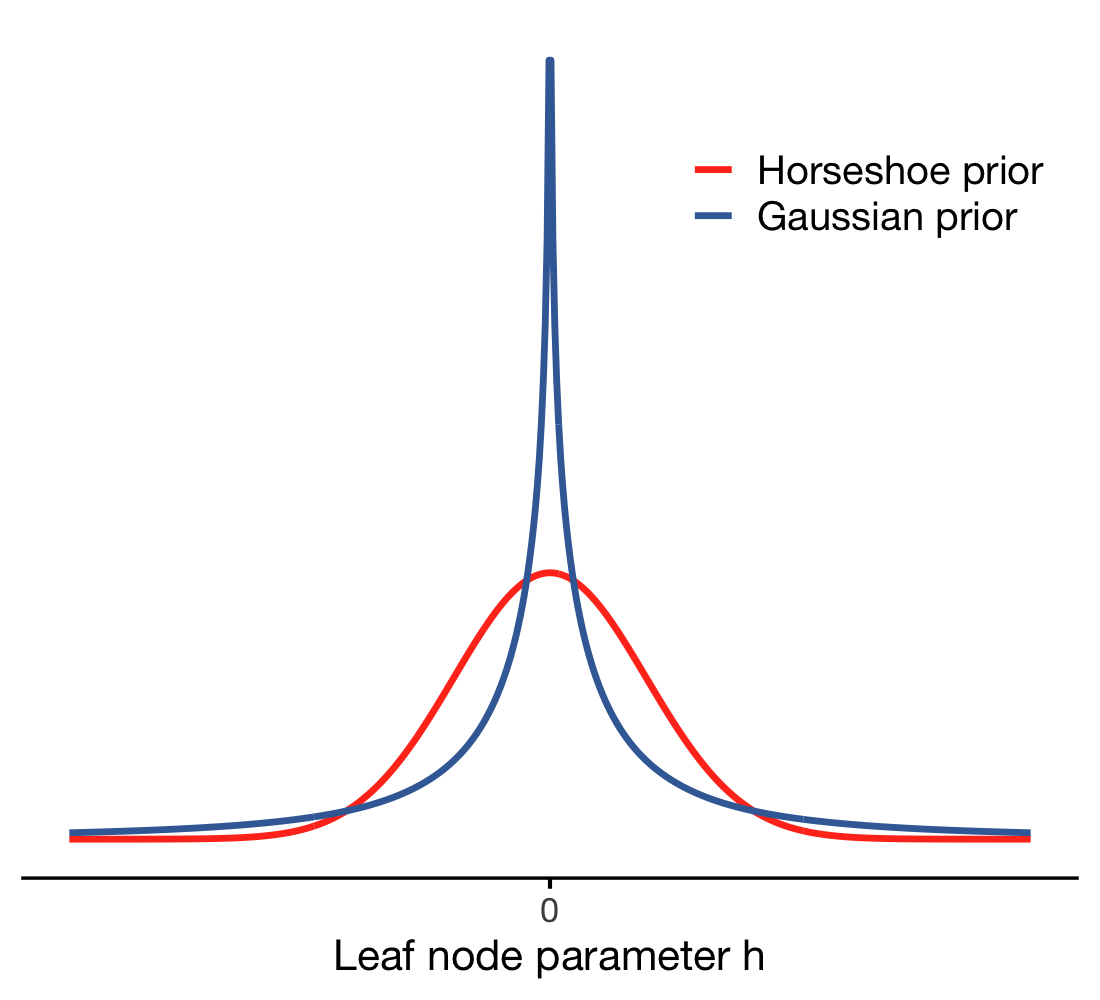
\includegraphics[width=\linewidth]{Horseshoe_plot_ICSDS.png}
\end{column}
\end{columns}
\end{frame}

%=========================================================
\section{Horseshoe Forests}
%=========================================================

%---------------------------------------------------------
\begin{frame}{The novel move: horseshoe on the step heights}
For a tree $\T$ with leaves $\ell = 1, \ldots, L$:
\[
h_\ell \mid \lambda_\ell^2, \gamma^2 \;\sim\; \N(0, \lambda_\ell^2\, \gamma^2),
\qquad
\lambda_\ell \sim \mathcal{C}^+(0,1), \quad \gamma \sim \mathcal{C}^+(0,1).
\]

\bigskip

\textbf{What changes from standard BART.}
\begin{itemize}
  \item Tree structure prior $p_\T$: unchanged Galton--Watson.
  \item Step-height prior: \alert{Gaussian $\to$ horseshoe}.
\end{itemize}

\bigskip

\textbf{Effect.} Regularisation migrates from \emph{where splits go} to \emph{how big each local effect is}:
\begin{itemize}
  \item Trees can split on \emph{any} covariate.
  \item Step heights are shrunk \emph{per leaf}.
  \item Real signals: leaves with large step heights. Noise: leaves with step heights near zero.
\end{itemize}
\end{frame}

%---------------------------------------------------------
\begin{frame}{Why this is better than DART for causal inference}
\textbf{DART} (Linero, 2018) regularises the \emph{tree structure}: a Dirichlet prior on splitting probabilities concentrates splits on a subset of covariates.

\bigskip

\begin{columns}[T,onlytextwidth]
\begin{column}{0.45\textwidth}
\textbf{Two problems.}
\begin{itemize}
  \item DART can concentrate on the \emph{wrong} subset — see green (true signal) being dropped in favour of red (noise) in different replications.
  \item Dropping a weak confounder violates unconfoundedness $\Rightarrow$ \alert{regularisation-induced confounding} (Hahn et al., 2018).
\end{itemize}

\bigskip

\textbf{Horseshoe forest.} Keeps every covariate split-eligible — shrinks the \emph{magnitudes} of the resulting leaf effects.
\end{column}
\begin{column}{0.55\textwidth}
\centering
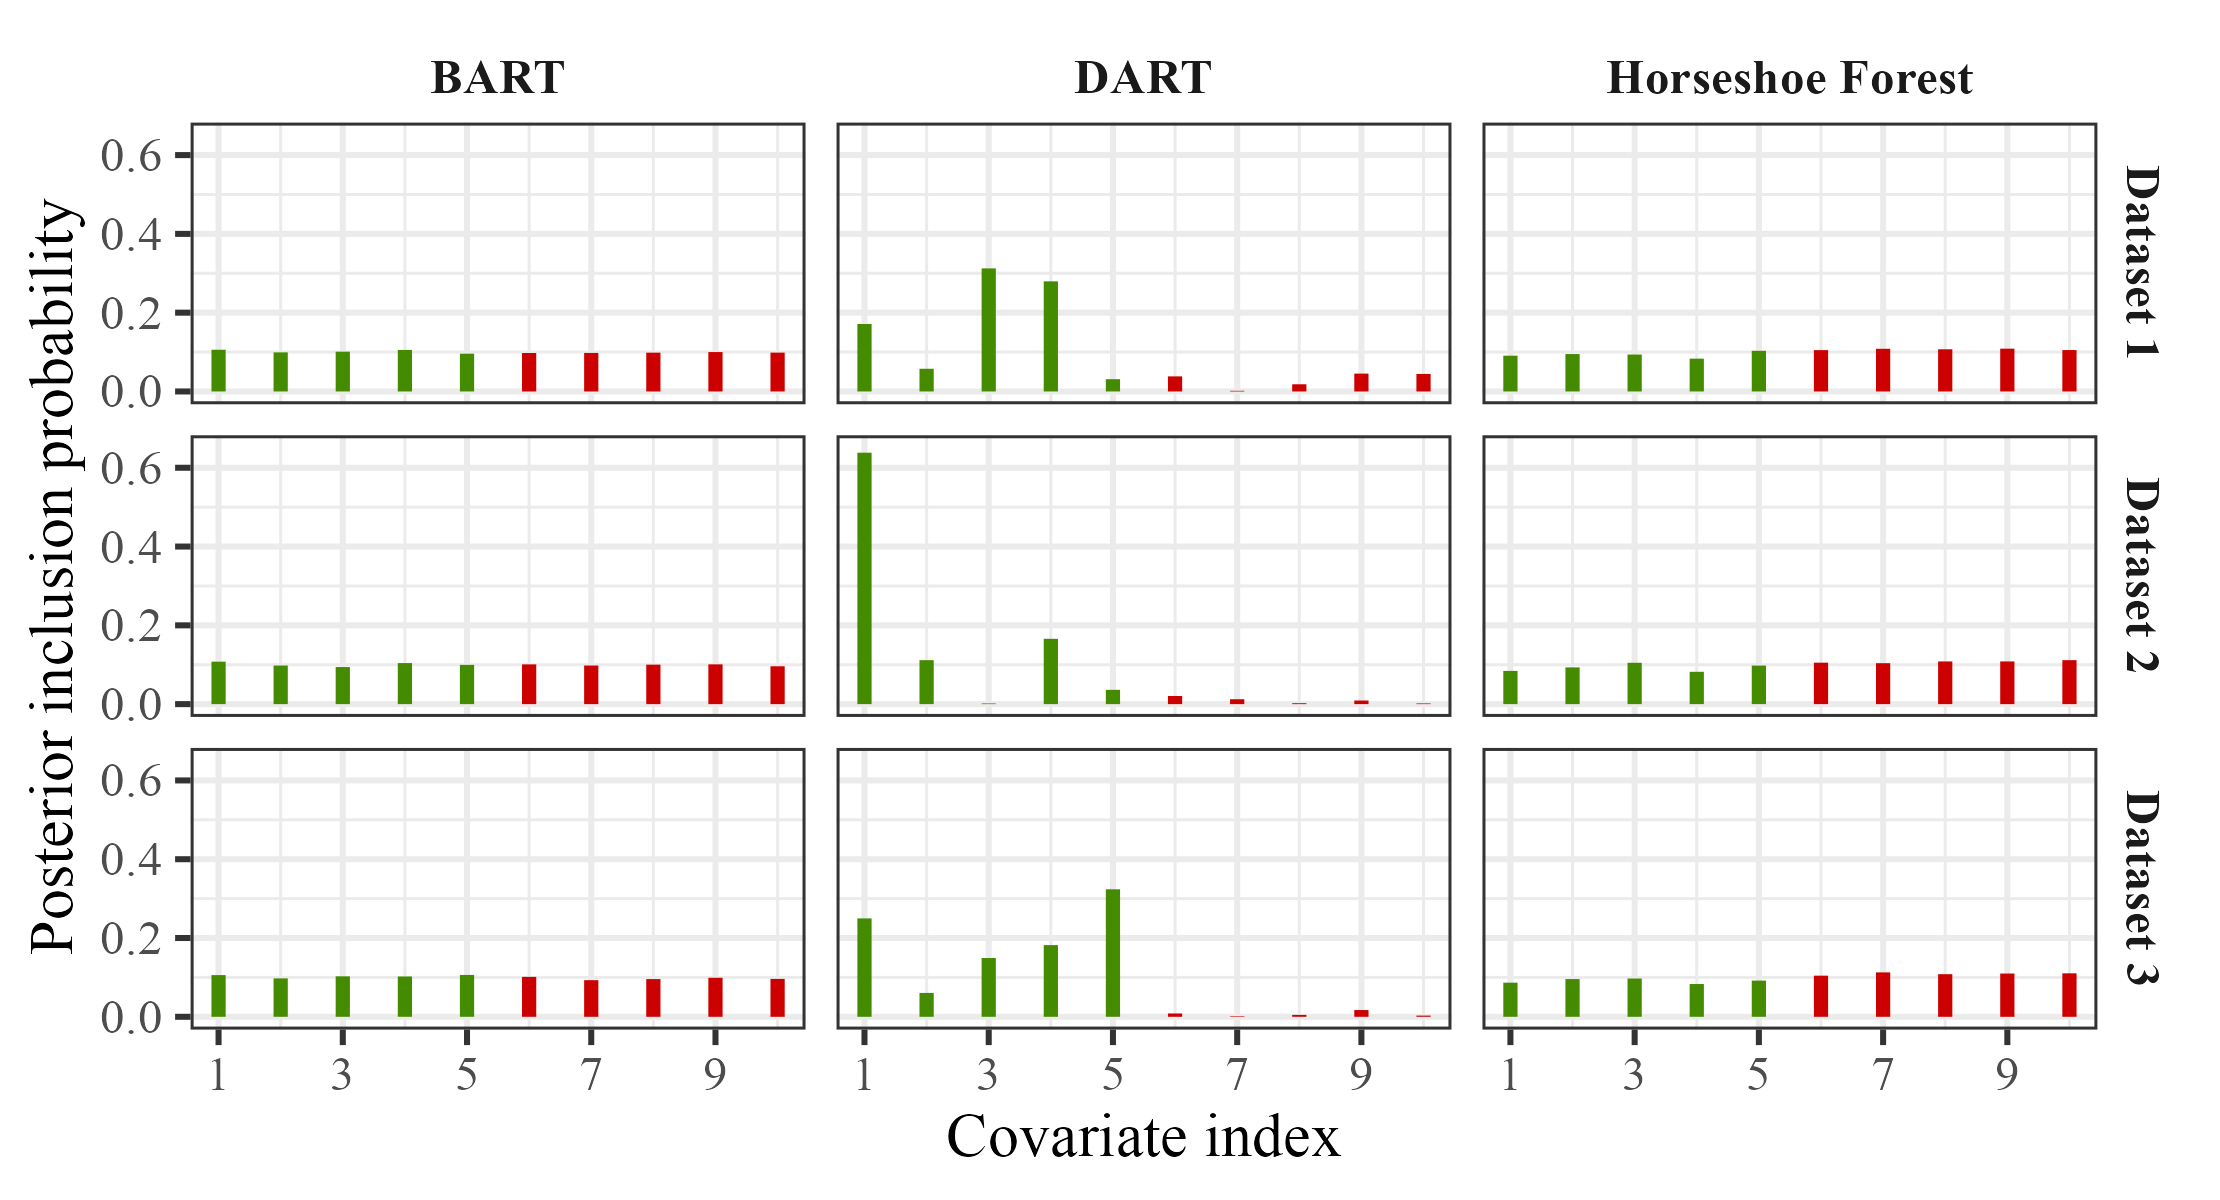
\includegraphics[width=\linewidth]{revision_posterior_inclusion_plot.png}
\end{column}
\end{columns}
\end{frame}

%=========================================================
\section{Posterior inference}
%=========================================================

%---------------------------------------------------------
\begin{frame}{Reversible-jump within Gibbs}
\begin{columns}[c,onlytextwidth]
\begin{column}{0.40\textwidth}
The horseshoe prior is \emph{not} Gaussian-conjugate $\Rightarrow$ step heights cannot be marginalised out.

\medskip

GROW and PRUNE moves change the dimension of $\Hh_j$. We use a \alert{reversible-jump} step with a tailored proposal for $(\T_j, \Hh_j)$.

\medskip

This sits inside a Gibbs sampler that updates the forests $f$ and $\tau$, the error variance $\sigma^2$, and the augmented censored event times.
\end{column}
\begin{column}{0.58\textwidth}
\centering
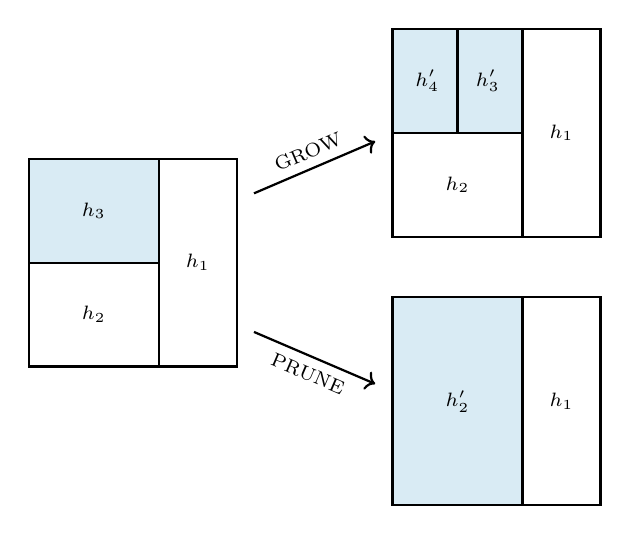
\begin{tikzpicture}[
  scale=1.1, every node/.style={font=\scriptsize}
]
% Parent partition
\fill[myaccent!15] (0,1.2) rectangle (1.5,2.4);
\draw[thick] (0,0) rectangle (2.4,2.4);
\draw[thick] (1.5,0) -- (1.5,2.4);
\draw[thick] (0,1.2) -- (1.5,1.2);
\node at (0.75,1.8) {$h_3$};
\node at (0.75,0.6) {$h_2$};
\node at (1.95,1.2) {$h_1$};

\draw[->, thick] (2.6,2.0) -- (4.0,2.6) node[midway, above, sloped] {GROW};
\draw[->, thick] (2.6,0.4) -- (4.0,-0.2) node[midway, below, sloped] {PRUNE};

% GROW result
\begin{scope}[shift={(4.2,1.5)}]
\fill[myaccent!15] (0,1.2) rectangle (1.5,2.4);
\draw[thick] (0,0) rectangle (2.4,2.4);
\draw[thick] (1.5,0) -- (1.5,2.4);
\draw[thick] (0,1.2) -- (1.5,1.2);
\draw[thick] (0.75,1.2) -- (0.75,2.4);
\node at (0.4,1.8) {$h'_4$};
\node at (1.1,1.8) {$h'_3$};
\node at (0.75,0.6) {$h_2$};
\node at (1.95,1.2) {$h_1$};
\end{scope}

% PRUNE result
\begin{scope}[shift={(4.2,-1.6)}]
\fill[myaccent!15] (0,0) rectangle (1.5,2.4);
\draw[thick] (0,0) rectangle (2.4,2.4);
\draw[thick] (1.5,0) -- (1.5,2.4);
\node at (0.75,1.2) {$h'_2$};
\node at (1.95,1.2) {$h_1$};
\end{scope}
\end{tikzpicture}
\end{column}
\end{columns}
\end{frame}

%---------------------------------------------------------
\begin{frame}{Censoring via data augmentation}
We follow Tanner \& Wong (1987): treat censored event times as latent variables in the Gibbs sampler.

\bigskip

At iteration $t$, for each censored $i$:
\[
\log T_i^{(t)} \;\sim\; \N\!\bigl(\hat\mu_i^{(t)},\, \sigma^{2,(t)}\bigr)
\quad \text{truncated to } (\log Y_i, \infty),
\]
where $\hat\mu_i^{(t)} = f^{(t)}\!\bigl(x_i, \hat e(x_i)\bigr) + a_i\, \tau^{(t)}(x_i)$.

\bigskip

\textbf{Net effect.} The sampler sees a fully-observed dataset on every iteration. The posterior averages over the uncertainty in the imputed event times.

\bigskip

\textbf{Propensity score.} Estimated separately with a \emph{binary-outcome} Horseshoe Forest (via probit augmentation), then plugged into the prognostic forest. Avoids feedback (Zigler, 2016); improves finite-sample bias (Hahn et al., 2020).
\end{frame}

%=========================================================
\section{Simulations}
%=========================================================

%---------------------------------------------------------
\begin{frame}{Simulation 1: CATE estimation as $p$ grows}
Non-linear treatment effect with sparse main (5\%) $+$ interaction (1\%) structure; $n = 200$, $p \in [50, 5000]$, censoring $\approx 35\%$.

\vspace{-0.2em}
\begin{center}
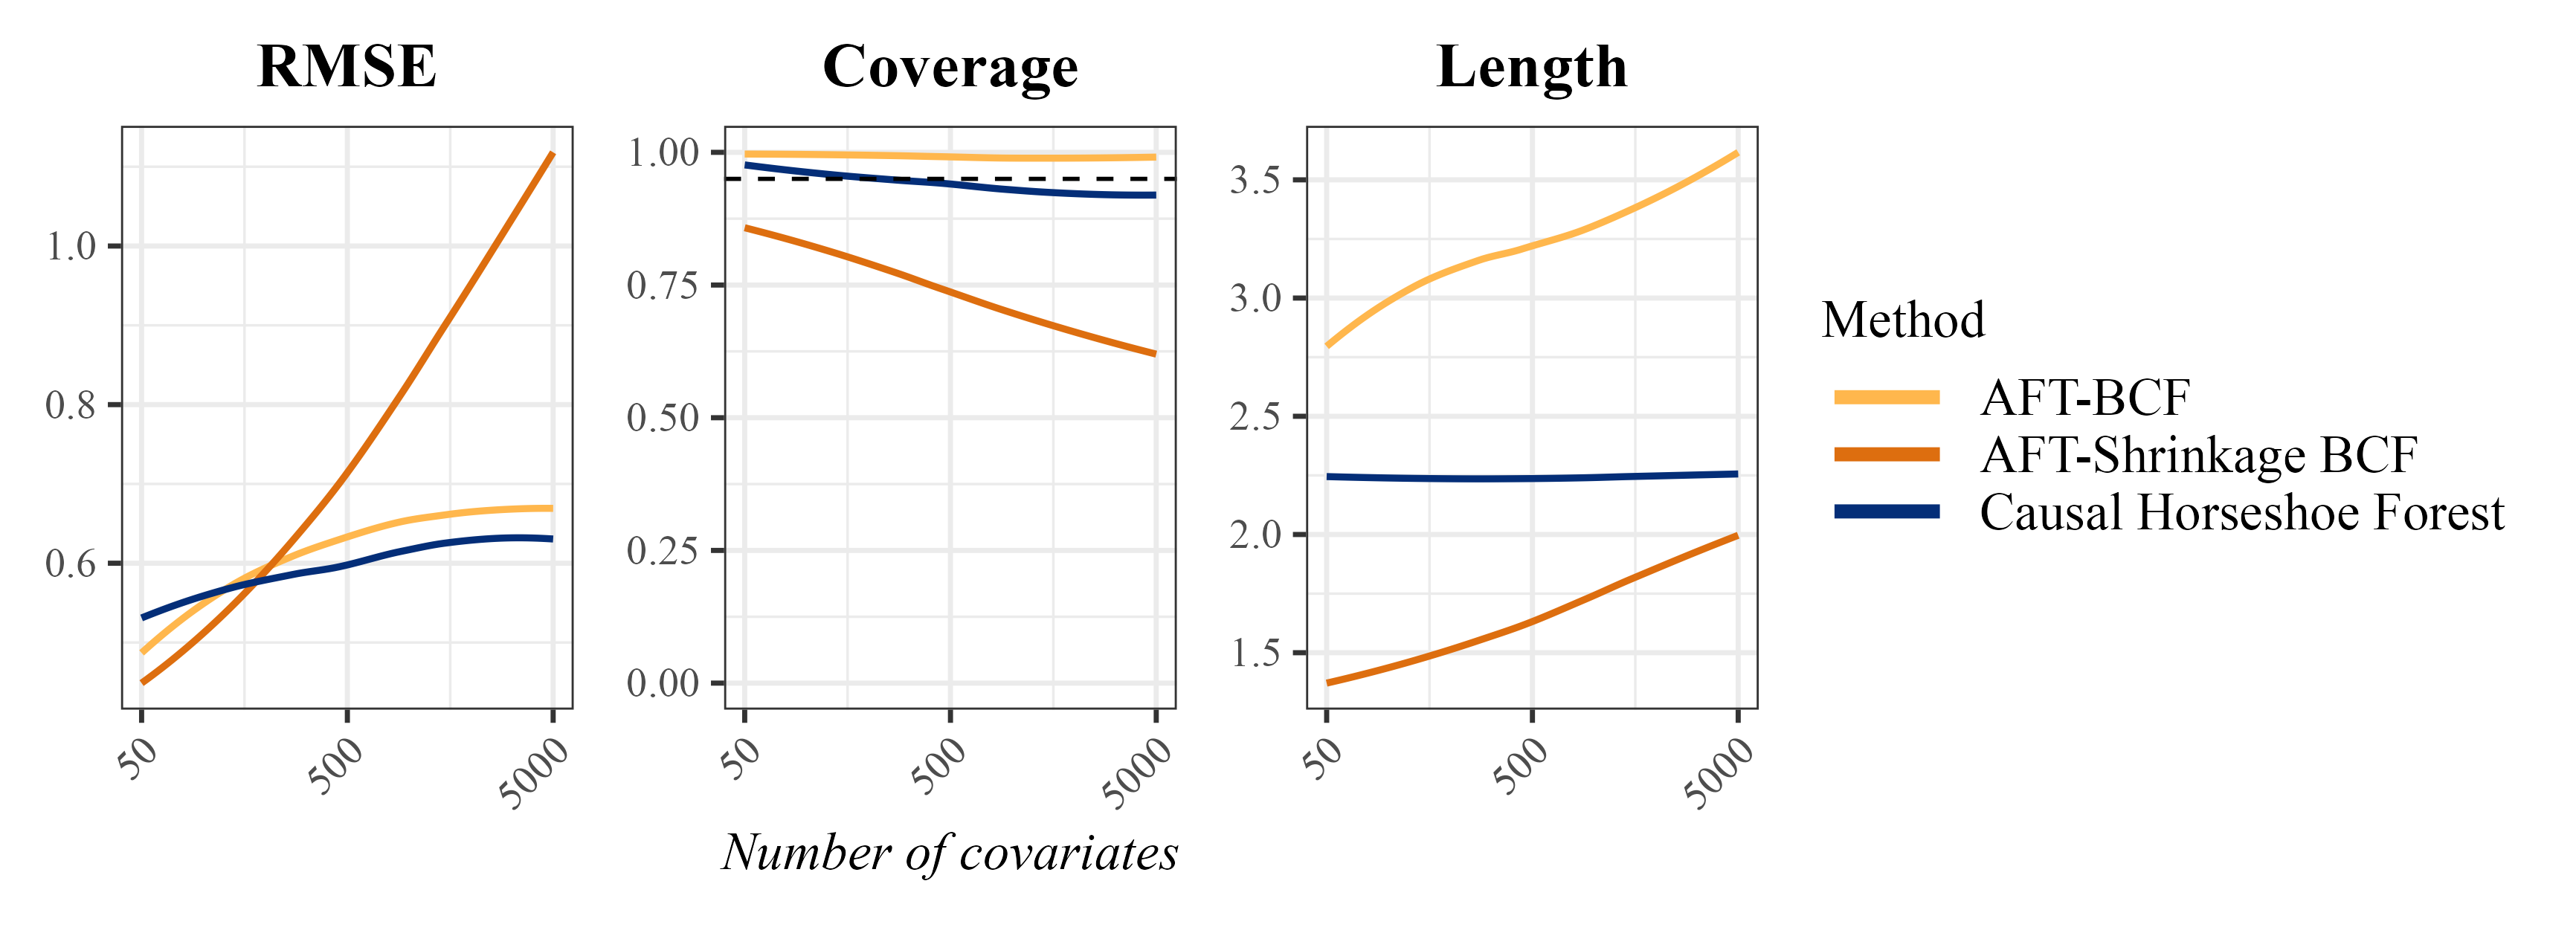
\includegraphics[width=0.92\linewidth]{revision_main_deeper.png}
\end{center}

\vspace{-0.2em}
\textbf{Punchline.} Causal Horseshoe Forest: stable RMSE, near-nominal coverage. AFT-BCF: coverage near 1 only because its credible intervals balloon.
\end{frame}

%---------------------------------------------------------
\begin{frame}{Simulation 2: regularisation-induced confounding}
$n = 100$, $p = 500$, censoring $\approx 35\%$. Two groups of confounders:
\begin{itemize}
  \item $|S| = 5$ \textbf{strong} confounders — strong on both treatment and outcome.
  \item $|W| \in \{1, \ldots, 20\}$ \textbf{weak} confounders — strong on treatment, weak on outcome.
\end{itemize}

\vspace{0.1cm}
\begin{center}
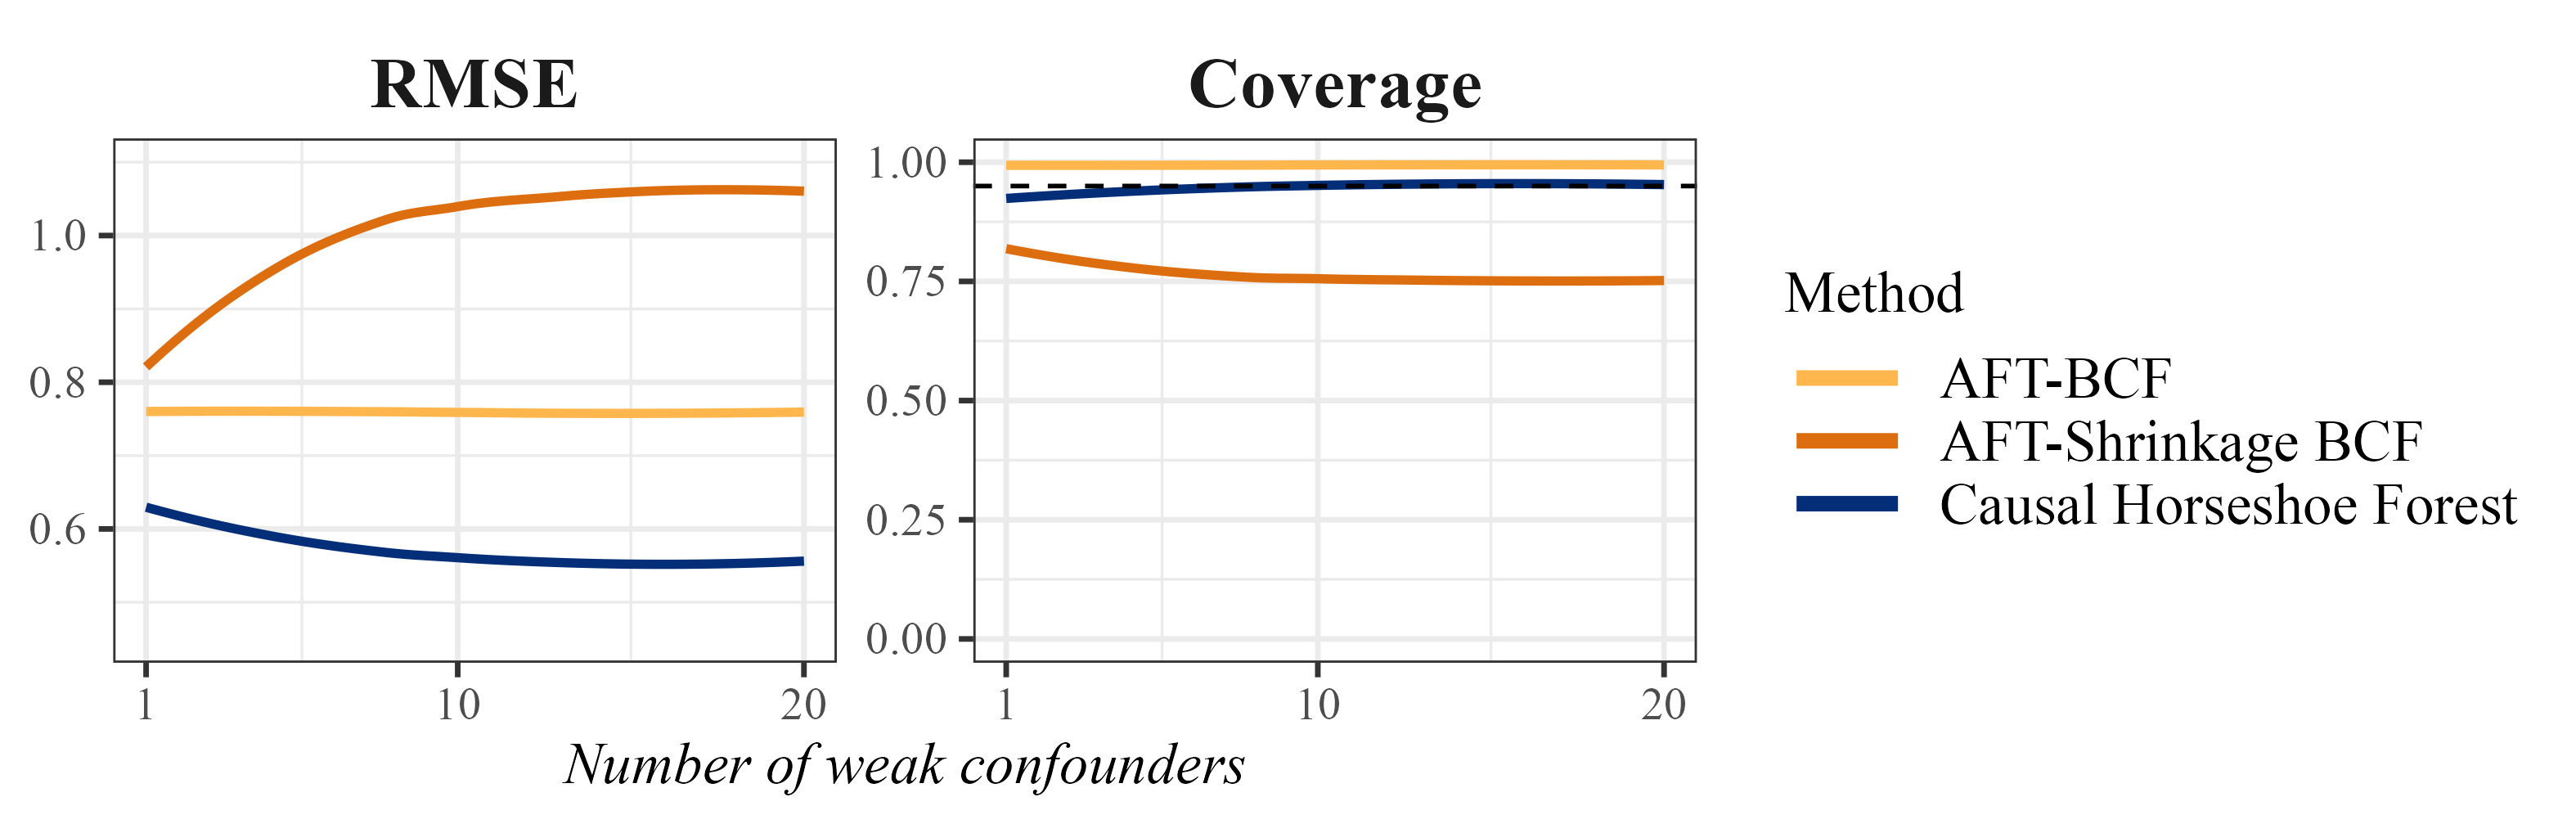
\includegraphics[width=0.92\linewidth]{revision_ric.png}
\end{center}

\vspace{-0.2em}
\textbf{Punchline.} Dirichlet-on-splits (AFT-Shrinkage BCF) drops weak confounders $\Rightarrow$ RMSE blows up. Horseshoe-on-step-heights is stable.
\end{frame}

%=========================================================
\section{Application: pancreatic cancer}
%=========================================================

%---------------------------------------------------------
\begin{frame}{PDAC: results}
\begin{columns}[c,onlytextwidth]
\begin{column}{0.5\textwidth}
\centering
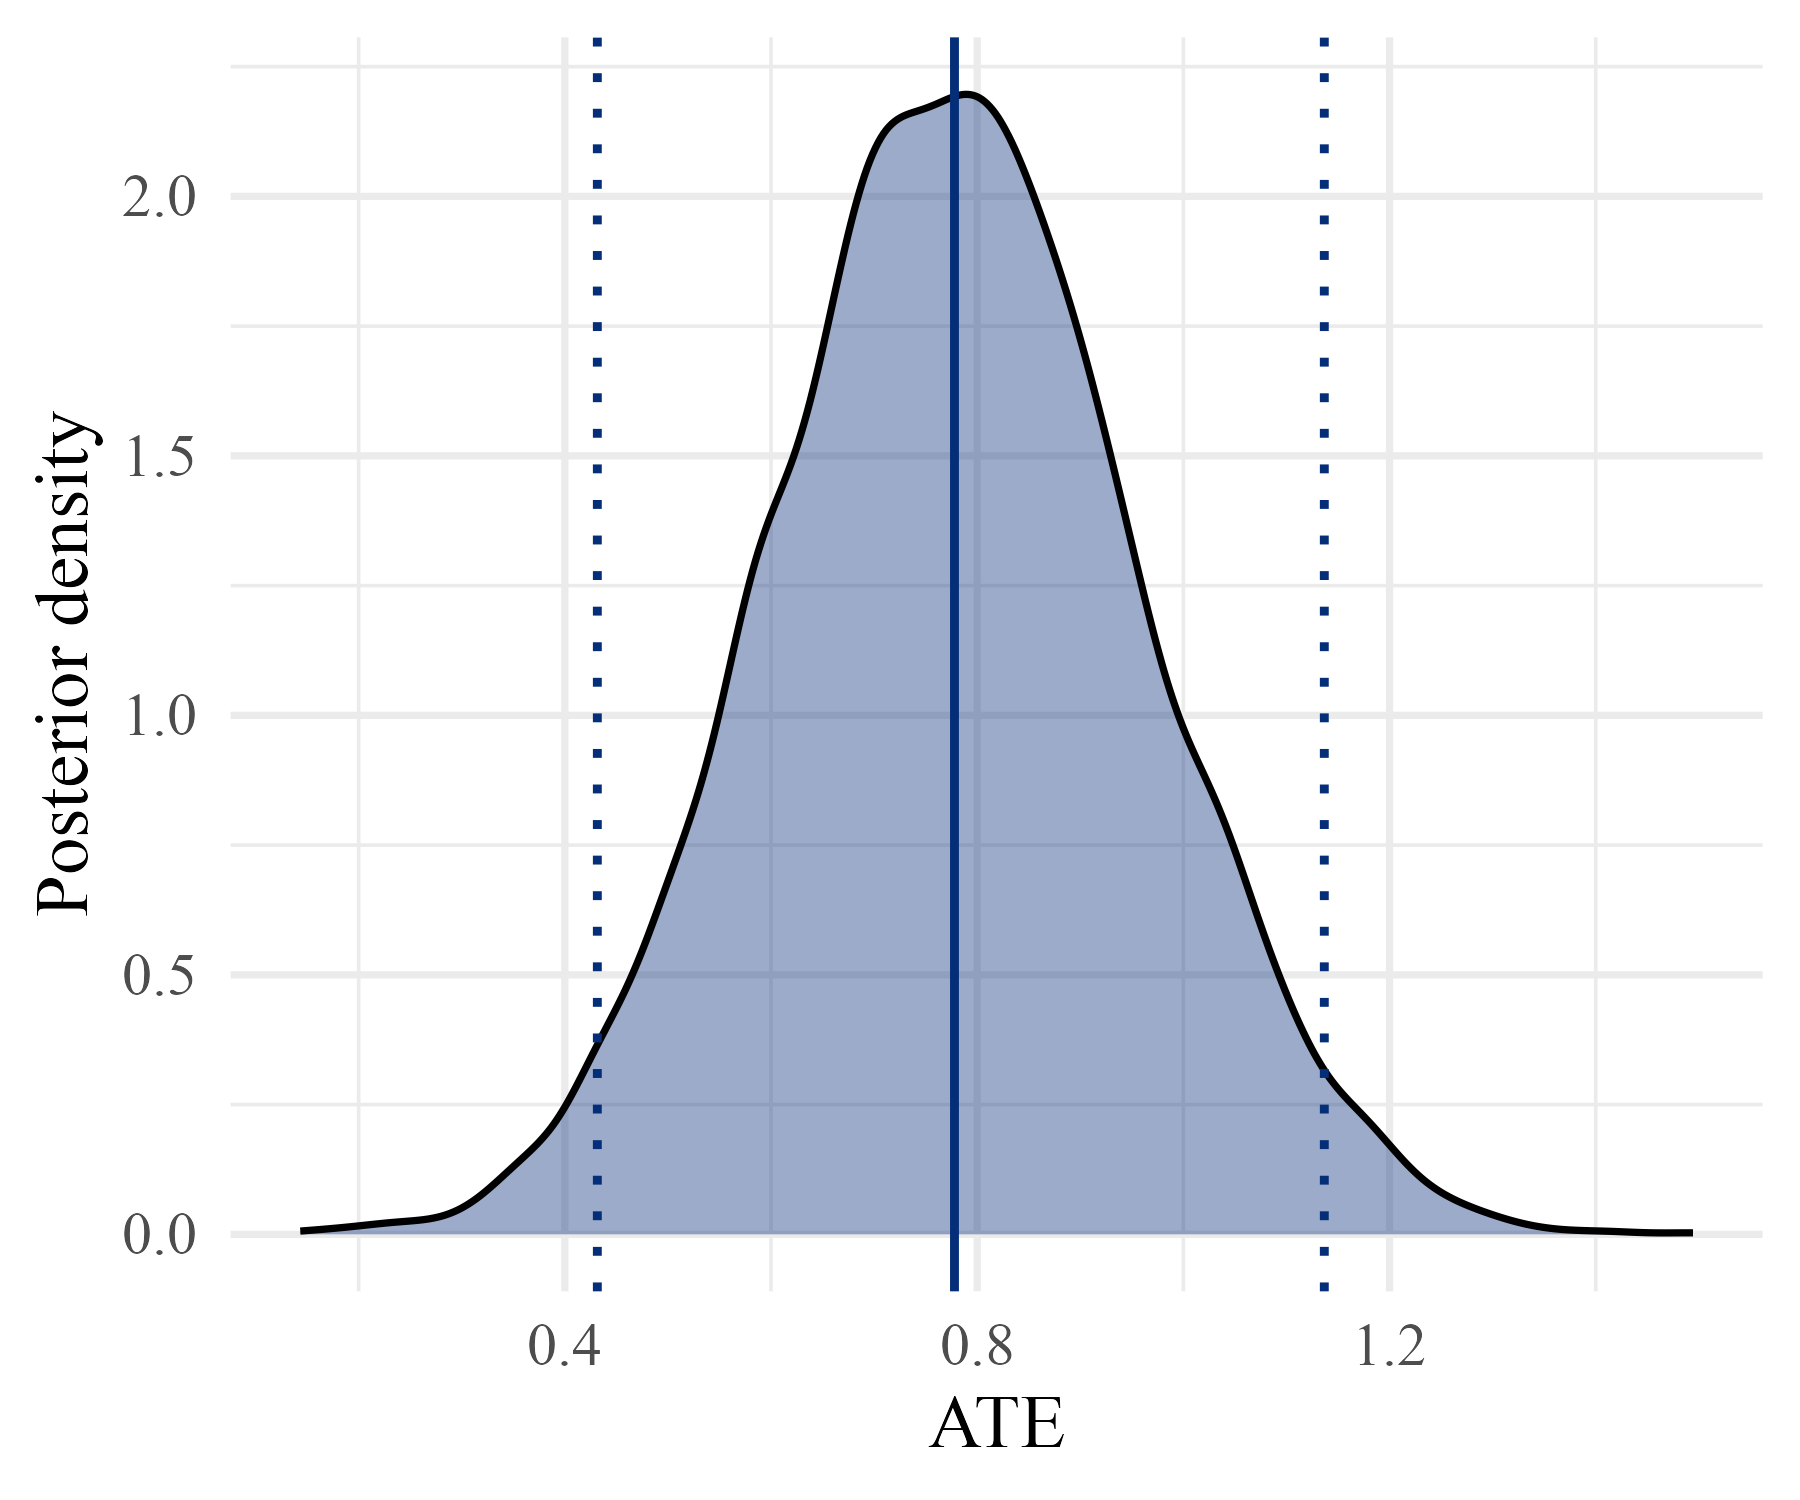
\includegraphics[width=\linewidth]{Plot_posteriorATE.png}

\smallskip
{\footnotesize $\widehat{\text{ATE}} \approx 0.75$,\, 95\% CrI $(0.40,\,1.11)$.\\
Acceleration factor $e^{0.75} \approx 2.1$ — expected survival roughly doubles.}
\end{column}
\begin{column}{0.5\textwidth}
\centering
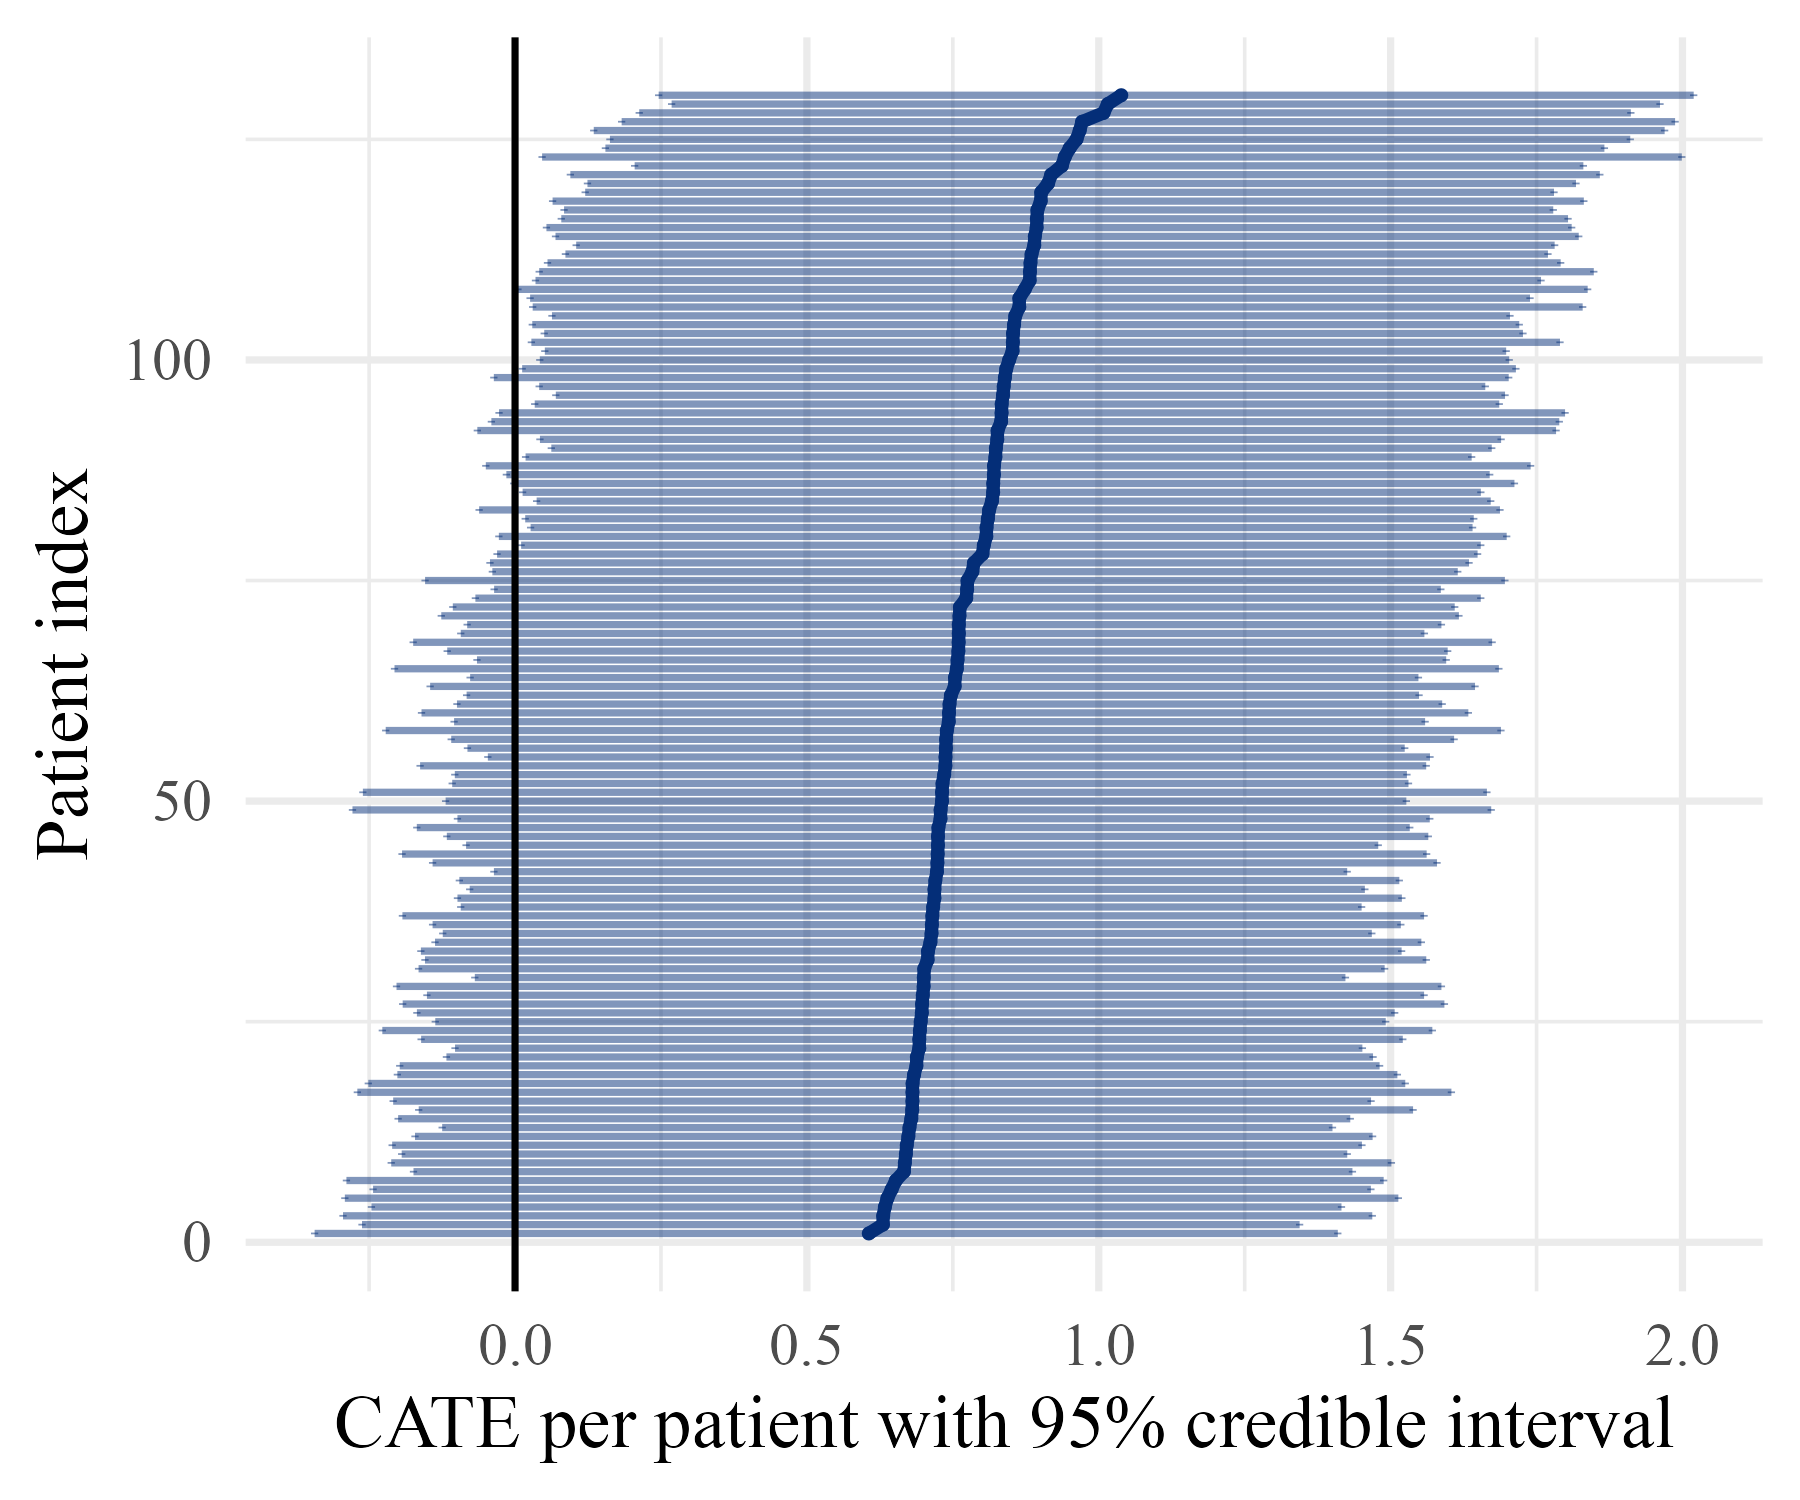
\includegraphics[width=\linewidth]{plot_CATEpatient.png}

\smallskip
{\footnotesize $\approx 96.9\%$ of patients have $P(\tau(X_i)>0\mid \text{data}) > 0.95$;\\
little evidence for between-patient heterogeneity.}
\end{column}
\end{columns}

\medskip

{\footnotesize \textbf{Caveats.} SUTVA not strictly met (regimens vary); positivity unverifiable when $p \gg n$; immortal-time bias may favour the treated group. Landmark sensitivity analysis in Suppl.~S.6.}
\end{frame}

%=========================================================
\section{Wrap-up}
%=========================================================

%---------------------------------------------------------
\begin{frame}{Take-aways}
\begin{itemize}
  \item \alert{Where you regularise matters.} Shifting regularisation from the tree \emph{structure} to the \emph{step heights} of a tree ensemble gives a flexible, adaptive prior for high-dimensional CATE estimation.
  \vspace{0.3cm}
  \item \alert{The price is a reversible-jump sampler.} A tailored tree proposal keeps the chain mixing well.
  \vspace{0.3cm}
  \item \alert{Strong empirical performance.} Stable RMSE and near-nominal coverage as $p$ grows; robust to regularisation-induced confounding where competing methods break down.
  \vspace{0.3cm}
  \item \alert{Available as software.} \texttt{ShrinkageTrees} on CRAN and GitHub.
\end{itemize}
\end{frame}

%---------------------------------------------------------
\begin{frame}{Thank you}
\begin{columns}[c,onlytextwidth]
\begin{column}{0.62\textwidth}
\begin{itemize}
  \item Preprint on arXiv: \texttt{2507.22004}.
  \item R package \textbf{ShrinkageTrees} on CRAN (and GitHub).
  \item Questions? \texttt{t.jacobs@vu.nl}.
\end{itemize}

\bigskip
\end{column}
\begin{column}{0.38\textwidth}
\centering
\qrcode[height=3cm]{https://tijn-jacobs.github.io/}

\smallskip
{\footnotesize \texttt{tijn-jacobs.github.io}}
\end{column}
\end{columns}

\vfill

\begin{columns}[c,onlytextwidth]
\begin{column}{0.68\textwidth}
\tiny
This project has received funding from the European Research Council (ERC) under the European Union's Horizon Europe program under Grant agreement No.\ 101074082. Views and opinions expressed are however those of the author(s) only and do not necessarily reflect those of the European Union or the European Research Council Executive Agency. Neither the European Union nor the granting authority can be held responsible for them.
\end{column}
\begin{column}{0.30\textwidth}
\centering
\includegraphics[width=\linewidth]{"EN-Funded by the EU-POS".jpg}
\end{column}
\end{columns}
\end{frame}

%=========================================================
\section{Additional slides}
%=========================================================

%---------------------------------------------------------
\begin{frame}{Simulation 1: data-generating process}
$n = 200$, censoring $\approx 35\%$, $p$ swept from $50$ to $5000$:
\[
X_i \sim \mathcal{U}[0,1]^p,\quad A_i \sim \mathrm{Ber}(e(x_i)),\quad
\log T_i \sim \N\!\bigl(f(x_i) + A_i \tau(x_i),\, \sigma^2\bigr).
\]
$e(x_i) = \Phi(-0.5 + 0.4 x_{i1} - 0.1 x_{i3} + 0.3 x_{i5})$; $\;f(x_i) = \beta_f^\top x_i$ with $\beta_f$ spike-and-slab.

\smallskip
\textbf{Treatment effect.} Friedman non-linear core $+$ sparse main effects $+$ sparse pairwise interactions,
\[
\tau(x_i) = 10\sin(\pi x_{i1} x_{i2}) + 20(x_{i3}-0.5)^2 + 10 x_{i4} + 5 x_{i5} + \beta_\tau^\top x_i + x_i^\top \Gamma x_i,
\]
with $\beta_\tau$ spike-and-slab ($s_{\mathrm{main}} = 0.05$) and sparse symmetric $\Gamma$ ($s_{\mathrm{int}} = 0.01$).
\end{frame}

%---------------------------------------------------------
\begin{frame}{Simulation 2: data-generating process}
$p = 500$, $n = 100$, $|S|=5$ strong confounders, $|W| \in \{1,\ldots,20\}$ weak confounders:
\begin{align*}
e(x_i)    &\propto \tfrac{1}{\sqrt{5+|W|}}\Bigl(\textstyle\sum_{j\in S} x_{ij} + 2 \sum_{j \in W} x_{ij}\Bigr), \\
f(x_i)    &= 4 \sum_{j\in S} x_{ij} + \sum_{j\in W} x_{ij}, \\
\tau(x_i) &= 1 + \sum_{j \in S} \beta_j\, x_{ij}.
\end{align*}
\end{frame}

%---------------------------------------------------------
\begin{frame}{Full conditional update of step heights}
Given the current tree $\T$ with $L$ leaves, encode the partition by $D \in \R^{n \times L}$. Then the conditional posterior of $h \in \R^L$ is
\[
h \;\sim\; \N_L\!\Bigl( \Omega^{-1} D^\top R,\;\Omega^{-1} \Bigr),
\qquad
\Omega = D^\top D + \bigl(\omega \gamma^2 \mathrm{diag}(\lambda_1^2, \ldots, \lambda_L^2)\bigr)^{-1}.
\]
Coordinate-wise:
\[
h_\ell \mid \cdot \;\sim\;
\N\!\left( \tfrac{\bar R_\ell}{n_\ell + 1/(\gamma^2 \lambda_\ell^2 \omega)},\;
            \tfrac{\sigma^2}{n_\ell + 1/(\gamma^2 \lambda_\ell^2 \omega)} \right).
\]

\bigskip

The shrinkage parameters update in closed form via the inverse-gamma auxiliary representation (Makalic \& Schmidt, 2016).
\end{frame}

%---------------------------------------------------------
\begin{frame}{Sparsity on splits can drop real signal}
{\footnotesize \textbf{Setup.} $n=500$, $p=10$; first 5 covariates carry strong signal, the rest are noise.}

\vspace{-0.3em}
\begin{figure}
\centering
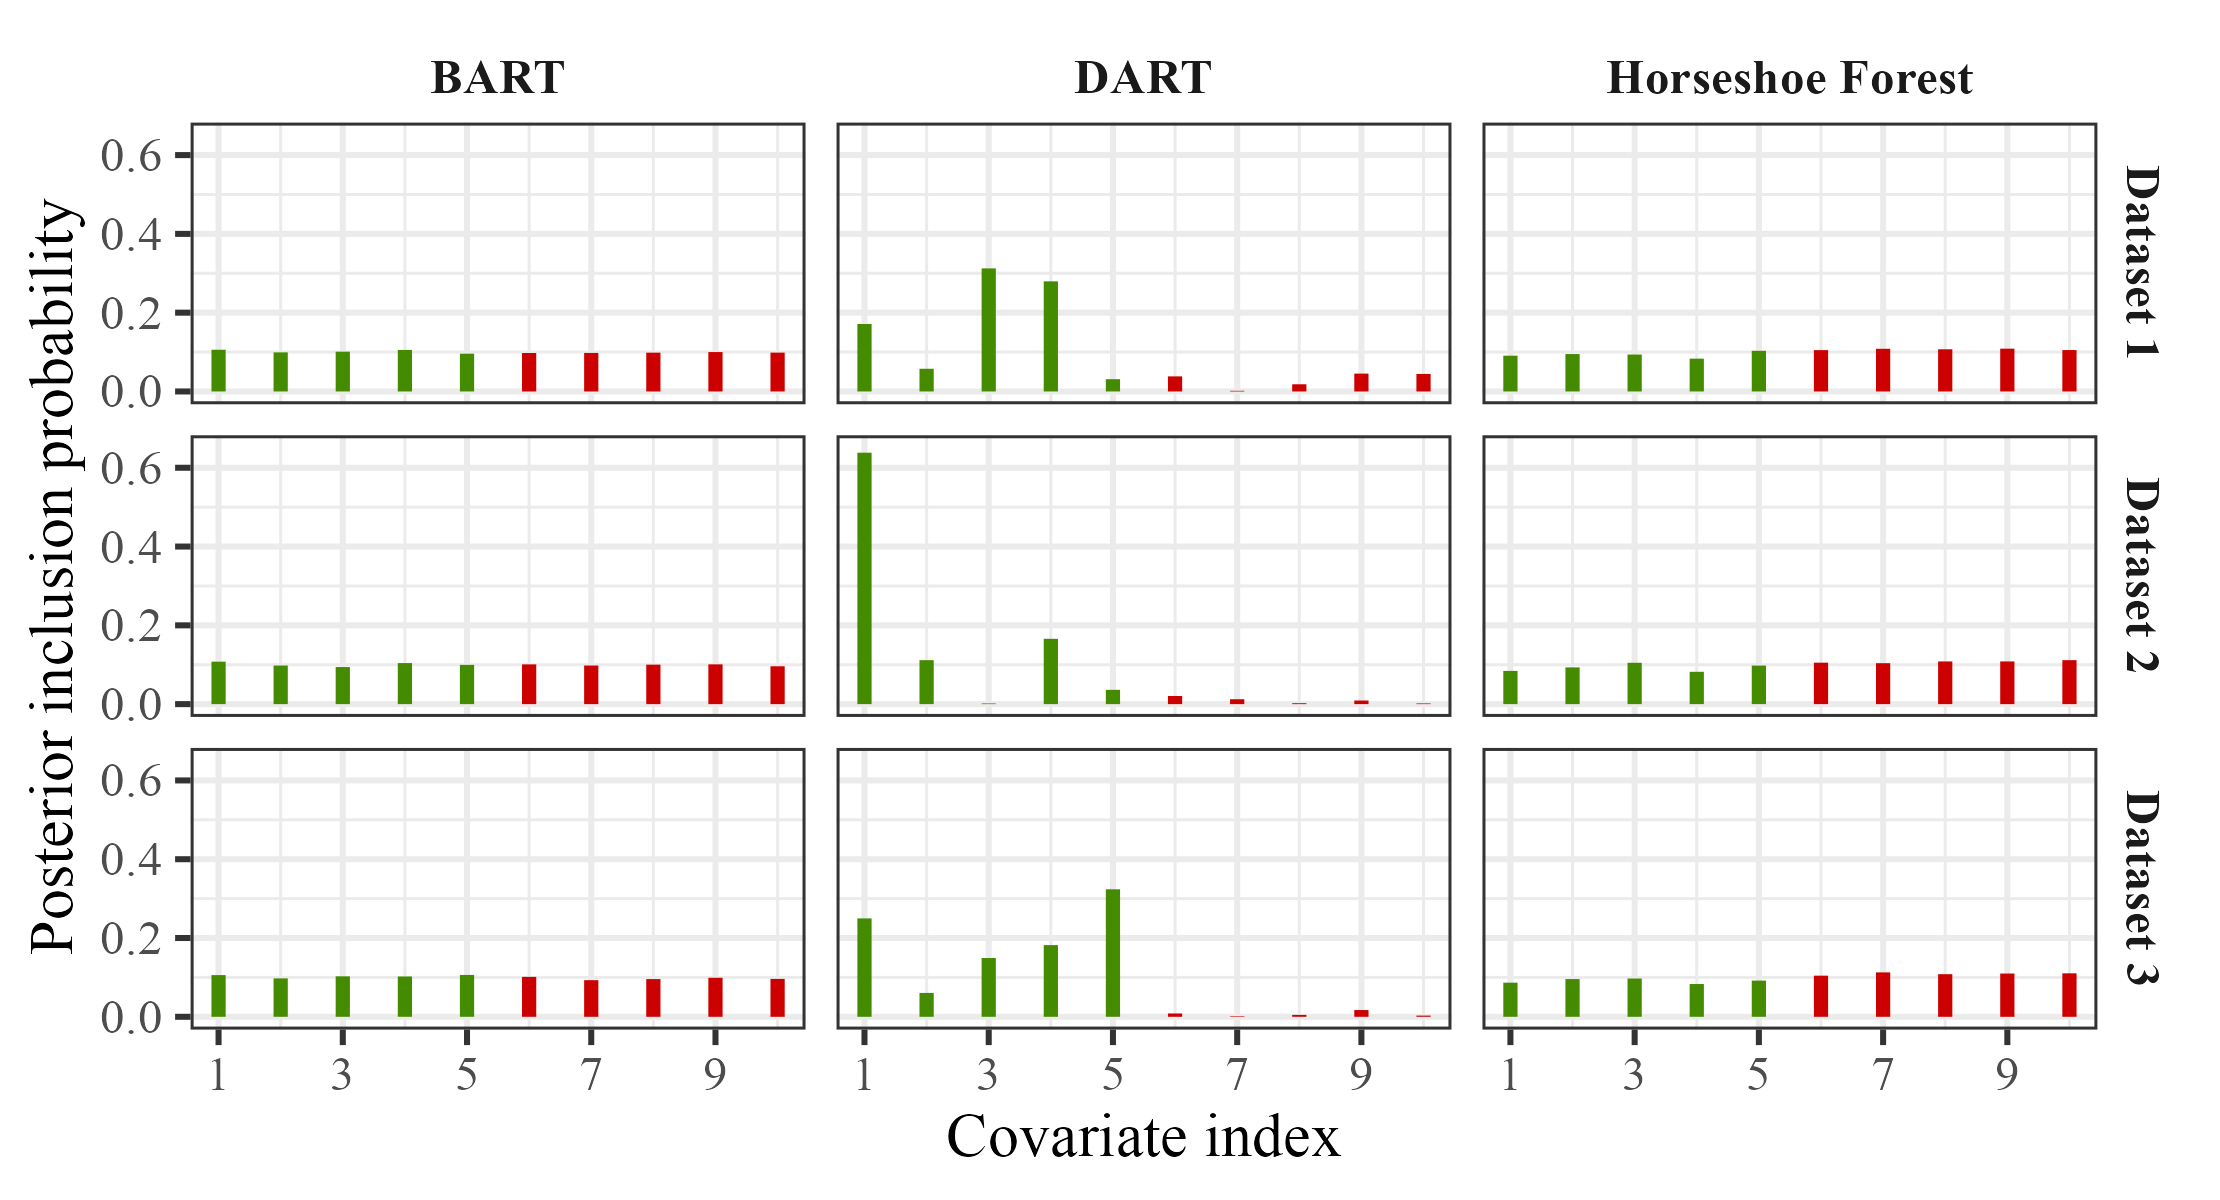
\includegraphics[width=0.72\linewidth]{revision_posterior_inclusion_plot.png}
\end{figure}

\vspace{-0.5em}
{\footnotesize
\begin{itemize}
  \item \textbf{BART} \& \textbf{Horseshoe Forest}: near-uniform splitting mass; horseshoe additionally shrinks noise step heights.
  \item \textbf{DART}: sharp concentration, but across replicates can land on the \emph{wrong} subset.
\end{itemize}}
\end{frame}

\end{document}
